\documentclass[12pt, letterpaper]{article}

% Font
\usepackage{amsmath, amssymb}
\usepackage{lmodern}
\usepackage{microtype}

% Format
\usepackage[letterpaper, margin = 1in]{geometry}
\setcounter{secnumdepth}{0}
\setlength{\parindent}{0.5in}
\usepackage[compact]{titlesec}
\titleformat*{\section}{\centering\normalfont\normalsize\bfseries}
\titleformat*{\subsection}{\raggedright\normalfont\normalsize\bfseries}
\titleformat*{\subsubsection}{\raggedright\normalfont\normalsize\bfseries\itshape}
\usepackage{indentfirst}

% References/Footnotes
\newcommand{\refsection}{\newpage \section{References}}
\usepackage[hang, flushmargin]{footmisc}

% Header
\usepackage{fancyhdr}
\pagestyle{fancy}
\fancyhf{}
\setlength{\headheight}{14.5pt}
\renewcommand{\headrulewidth}{0pt}
\fancyhead[L]{ DOUBLE STANDARDS }
\fancyhead[R]{\thepage}

% Links
\usepackage[colorlinks = true, linkcolor = black, urlcolor = black, citecolor = black]{hyperref}
\usepackage{xurl}

% Figures
\usepackage{graphicx}
\usepackage[labelfont = bf, font = small, labelsep = newline, singlelinecheck = false]{caption}

% Tables
\usepackage{booktabs}
\usepackage{tabularx}

% Lists
\providecommand{\tightlist}{%
  \setlength{\itemsep}{0pt}\setlength{\parskip}{0pt}}

% References
\newenvironment{CSLReferences}[2]{}{}

% Line spacing
\usepackage[doublespacing]{setspace}

\begin{document}

\section{Abstract}

\noindent Collective action is a powerful force driving social change
but often sparks contention about what actions are acceptable means to
effect social change. Five studies (total \(N = 2,979\)) investigated
double standards in judging collective action---that is, whether
observers judge the same protest actions to be more acceptable depending
on who the protesters are and what they are protesting. Two studies used
item response theory to develop an instrument of 25 controversial
protest actions to measure where people draw the line between acceptable
and unacceptable forms of collective action. Three preregistered
experiments found no consistent evidence for ingroup bias in terms of
social class when judging protests for workers' rights (Experiment 1),
in terms of race when judging protests for and against defunding the
police (Experiment 2), and in terms of gender when judging protests for
and against restricting abortion (Experiment 3). Instead, we found that
participants who identified as left-wing/liberal (Experiments 1--3) and
rejected system-justifying beliefs (Experiments 1--2) considered the
same protest actions more acceptable when a cause aligned with their
ideological orientation (for workers' rights, for defunding the police,
against restricting abortion) than when it did not (against defunding
the police, for restricting abortion). Conservative participants
considered the same actions somewhat more acceptable when protesters
supported, rather than opposed, restricting abortion (Experiment 3) but
considered all protest actions, for and against defunding the police,
equally unacceptable (Experiment 2). Our findings have theoretical and
practical implications for understanding the often-divided response to
social movements.

\textit{Keywords:} collective action, double standards, social identity
theory, system justification theory, partisanship, Black Lives Matter,
abortion

\vfill

\begin{center}
\noindent 11,654 words
\end{center}

\vfill

\section{Public Significance Statement}

\noindent This research shows that what people consider an acceptable
\emph{means} of protest depends on what the \emph{end} of a protest is.
That is, observers sometimes judge the \emph{same} controversial protest
action (e.g., blocking a road) to be more acceptable when the
protesters' cause (e.g., defunding the police) aligns with their own
ideological position. Conservatives, who support social order and oppose
social change, tend to consider all protest actions less acceptable than
progressives. Progressives, in turn, tend to consider disruptive but
non-violent actions acceptable means to achieve social change and
challenge social injustice. This finding helps explain the often-divided
response to recent protest movements.

\newpage

\section{ Double Standards in Judging Collective Action }

Protest movements often spark contention about what actions are
acceptable means of protest. Reactions to Black American athletes
kneeling during the national anthem to protest racist police violence
are a case in point. Kneeling during the national anthem is not violent,
disruptive, or illegal. And yet, only 29\% of White Americans (compared
to 66\% of Black Americans) and 11\% of Republicans (compared to 59\% of
Democrats) considered it appropriate for Black athletes to protest in
this way (YouGov, 2017). This and other examples suggest that \emph{who}
the protesters are and \emph{what} they are protesting influences how
acceptable their actions are judged to be.

In this paper, we examine double standards in judging collective
action---that is, whether observers judge the \emph{same} protest
actions as more or less acceptable depending on their own and the
protesters' group memberships \emph{or} on the protesters' cause and how
it aligns with their own ideological positions.

\hypertarget{double-standards-in-judging-collective-action}{%
\subsection{Double Standards in Judging Collective
Action}\label{double-standards-in-judging-collective-action}}

Collective action---that is, any action taken by group members to
advance a shared political goal (for similar definitions, see Becker,
2012; van Zomeren, 2016)---is a powerful force driving social change.
For example, Black Lives Matter protests shifted public discourse about
racial inequity toward antiracist ideas (Dunivin et al., 2022).

Collective action can take many forms. Psychologists distinguish between
\emph{normative} collective action that seeks to achieve a political
goal while conforming to the norms of the existing social system and
\emph{non-normative} collective action that violates those norms (Becker
\& Tausch, 2015; Wright et al., 1990). Some instead refer to the two
kinds of collective action as moderate and radical collective action
(e.g., Jiménez-Moya et al., 2015). Broadly, this distinction captures
the intuition that there are some forms of collective action that are
generally considered acceptable and others that are not.

Recent research has shown that this distinction matters for how people
respond to collective action (for a review, see Shuman et al., 2023).
Shuman et al. (2021) showed that non-normative, non-violent collective
action is more effective than either normative or violent collective
action at gaining concessions from those most resistant to social
change. Feinberg et al. (2020) demonstrated, however, that observers are
less supportive of social movements that use extreme protest
actions.\footnote{In contrast, White Americans exposed to pictures of
  destructive Black Lives Matter protests were not, on average, any less
  supportive of systemic change than those exposed to pictures of
  peaceful protests (Teixeira et al., 2022).} Similarly, Teixeira et al.
(2020) found that advantaged-group members perceive non-normative
collective action by disadvantaged-group members as more damaging to
their ingroup's social image and are thus less supportive of such
action. This means that activists face the dilemma that non-normative
collective action might be most effective at gaining concessions but
that it also risks reducing popular support for a cause. Together, these
studies show that the distinction between normative and non-normative
collective action is psychologically and societally consequential.

Past research has, for the most part, relied on ad-hoc distinctions
between what researchers themselves considered normative and
non-normative collective action. In liberal democracies, researchers
tend to consider actions such as signing petitions, voting in elections,
or peaceful protest to be normative and actions such as blocking
traffic, damaging property, or violent protest to be non-normative. But,
as reactions to Black athletes kneeling in protest suggest, the same
action might be considered acceptable by some and unacceptable by
others. In this research, we test for double standards in where people
draw the line between what is an acceptable (normative) and an
unacceptable (non-normative) form of collective action.\footnote{In this
  research, we use \emph{acceptable} (``agreed or approved of by most
  people in a society,'' Oxford Advanced Learner's Dictionary, n.d.) as
  a plain-language synonym for \emph{normative} (``conforming to the
  norms of the existing social system'').} For that purpose, we define a
double standard as judging the same protest actions as more or less
acceptable depending on who the protesters are and what they are
protesting (for a similar definition, see Foschi, 2000).\footnote{Feinberg
  et al. (2020) provided incidental evidence for double standards in
  judging collective action as, in a manipulation check, Black
  participants rated Black Lives Matter protests as less extreme than
  White participants and liberal participants rated protest actions for
  progressive causes as less extreme than conservative participants.}

\hypertarget{group-based-double-standards}{%
\subsubsection{Group-Based Double
Standards}\label{group-based-double-standards}}

Far more Black (\(66\%\)) than White (\(29\%\)) Americans considered it
appropriate for Black athletes to kneel during the national anthem to
protest racist police violence (YouGov, 2017). This suggests that what
protest actions people consider acceptable might depend on their own and
the protesters' group memberships.

Social Identity Theory (Tajfel \& Turner, 1979; for a recent review, see
Reimer et al., 2022) argues that just as people show self-serving biases
to achieve positive self-esteem, they show ingroup-serving biases to
achieve positive social identities. In other words, they think about
ingroup and outgroup in ``me''--``not me'' terms and favor ingroup
members (``us'') over outgroup members (``not us,'' Brewer, 2007).

One domain in which ingroup bias manifests is judgments about other
people's actions. Hewstone (1990) reviewed research showing that people
make ingroup-serving causal attributions when judging actions by ingroup
and outgroup members. For example, people tend to attribute negative
behavior by outgroup members to internal causes but attribute negative
behavior by ingroup members to external causes (see Pettigrew, 1979).
Valdesolo \& DeSteno (2007) demonstrated that participants judged the
same selfish action as less unfair when performed by themselves or an
ingroup member than when performed by an outgroup member. Other studies
(Abrams et al., 2013; Endevelt et al., 2021; for exceptions, see Mendoza
et al., 2014; Pinto et al., 2010) provided further evidence for ingroup
bias in judging moral transgressions by ingroup and outgroup members.

In the same vein, we propose that ingroup bias results in double
standards in judging collective action by ingroup and outgroup members.
That is, we hypothesize that people will judge the same protest actions
as more acceptable if the protesters are ingroup members and if the
cause of the protest aligns with the ingroup's interests. Notably, this
hypothesis applies equally to historically disadvantaged groups
mobilizing against social injustice and to historically advantaged
groups defending their group's position.

\hypertarget{ideology-based-double-standards}{%
\subsubsection{Ideology-Based Double
Standards}\label{ideology-based-double-standards}}

Far more Democrats (\(59\%\)) than Republicans (\(11\%\)) considered it
appropriate to kneel during the national anthem to protest racist police
violence (YouGov, 2017). This suggests that what protest actions people
consider acceptable might depend on the protesters' cause and how it
aligns with their own ideological positions.

One explanation for ideology-based double standards is that they result
from the same intergroup processes as other group-based double
standards. In this view, political partisanship functions as a social
identity (Finkel et al., 2020; Harris et al., 2022) and results from
universal cognitive mechanisms for forming, detecting, and maintaining
alliances (Pinsof et al., 2023). Like other identities, political
identities result in group-serving biases in how we evaluate ingroup and
outgroup members. This explanation aligns with Verkuyten et al.'s (2022)
finding that participants were more tolerant of transgressive protest
actions (e.g., sending hate mail) when taken by their most-liked, rather
than their least-liked, political group (e.g., climate activists).

Another explanation for ideology-based double standards is that they are
rooted in ideological differences in how conservatives and progressives
relate to social change and social inequality which, in turn, are
motivated by epistemic, existential, and relational needs (Jost et al.,
2003; Jost, 2021). As motivated social cognition, ideological
differences shape how we think and feel about political issues, actions,
and events. In this view, ideology-based double standards depend on
whether the cause of a protest aligns with someone's ideological
positions.

System Justification Theory (Jost et al., 2004; for a recent review, see
Jost, 2020), in particular, argues that people are motivated to defend,
justify, and bolster the prevailing social, economic, and political
system because doing so serves basic epistemic, existential, and
relational needs. Both advantaged and disadvantaged groups are thought
to be motivated to justify the existing system, although the strength of
this motivation and its expression vary across individuals and
situations. Conservatives, far more so than progressives, endorse
system-justifying beliefs.

While system justification often leads people to resist social change,
its relationship to collective action depends on the goal of the action.
Jost et al. (2017) argued that research on collective action needs to
distinguish between system-challenging protest aimed at changing an
unequal status quo and system-supporting protest aimed at maintaining or
defending an unequal status quo. Osborne et al. (2019) showed that, for
members of both advantaged and disadvantaged groups, system
justification is associated with supporting system-supporting actions
but with opposing system-challenging actions.

Just as system justification affects support for, and opposition to,
collective action, we propose that it results in ideology-based double
standards in what actions people consider acceptable forms of collective
action. That is, we hypothesize that people will judge the same protest
actions as more acceptable if they endorse system-justifying beliefs and
the protest supports the system or if they reject system-justifying
beliefs and the protest challenges the system.

In principle, the two explanations for ideology-based double
standards---in terms of intergroup processes and ideological
differences---could be disentangled by separating political identities
and causes. An explanation in terms of intergroup processes posits that
political identities, not causes, shape partisan behavior. Indeed,
research suggests that partisans' policy preferences depend more on the
stated position of their party than policy content (Cohen, 2003). An
explanation in terms of ideological differences instead posits that
there is an ``elective affinity'' between political causes and the
psychological needs and motives of their supporters (Jost, 2021). In
other words, the content of political ideologies is not arbitrary or a
historical accident, as implied by an explanation in terms of intergroup
processes (see Pinsof et al., 2023). In practice, however, the two
explanations are difficult to disentangle in the context of real-world
protest movements in which political identities and causes can seldom be
separated.

For now, we use ``group-based'' to refer to double standards based on
ascribed categories such as class, race, and gender and
``ideology-based'' to refer to double standards based on ideological
alignment. We compare the evidence for different explanations of those
double standards in the General Discussion.

\hypertarget{using-item-response-theory-to-detect-double-standards}{%
\subsection{Using Item Response Theory to Detect Double
Standards}\label{using-item-response-theory-to-detect-double-standards}}

Item response theory is a conceptual and statistical framework for
understanding how the characteristics of both items and respondents
shape responses to a set of items (DeMars, 2010). When respondents judge
whether each of a set of actions is an acceptable means of protest (1 =
\emph{yes}, 0 = \emph{no}), a two-parameter logistic item response
theory model estimates responses as a function of several latent
(unobserved) parameters:
\[ \Pr ( y_\textit{ij} = 1 ) = \text{logit}^{-1} ( \alpha_i ( \theta_j + \beta_i ) ) \]
where \(\Pr ( y_\textit{ij} = 1 )\) is the probability that respondent
\(j\) considers action \(i\) an acceptable means of protest,
\(\theta_j\) estimates how \emph{accepting} respondent \(j\) is of
various protest actions, \(\beta_i\) estimates how \emph{acceptable}
action \(i\) is, and \(\alpha_i\) estimates how \emph{discriminating}
action \(i\) is.

Figure \ref{fig:f1} illustrates those relationships for three
hypothetical protest actions. \(\theta_{(z)}\) is the
\emph{z}-standardized tendency for a participant to be more accepting of
various actions so that \(\beta_i\) determines the probability that the
average respondent (\(\theta_{(z)} = 0\)) considers an action an
acceptable means of protest. Action 2 (\(\beta_2 = 1.28\)) is more
acceptable than Actions 1 and 2 (\(\{ \beta_2, \beta_3 \} = 0\)) as the
average respondent is more likely to consider the former (\(\Pr = .78\))
than the latter (\(\Pr = .50\)) acceptable means of protest. Action 3
(\(\alpha_3 = 3.60\)) is more discriminating than Actions 1 and 2
(\(\{ \alpha_1, \alpha_2 \} = 1\)) as the slope for the relationship
between how accepting a respondent is and how likely they are to
consider an action acceptable is steeper for the former action. This
means that knowing whether someone considers Action 3 acceptable
provides more information about them than knowing whether they consider
Actions 1 or 2 acceptable.

\begin{figure}
\centering
\caption{Item response curves for three hypothetical protest actions}
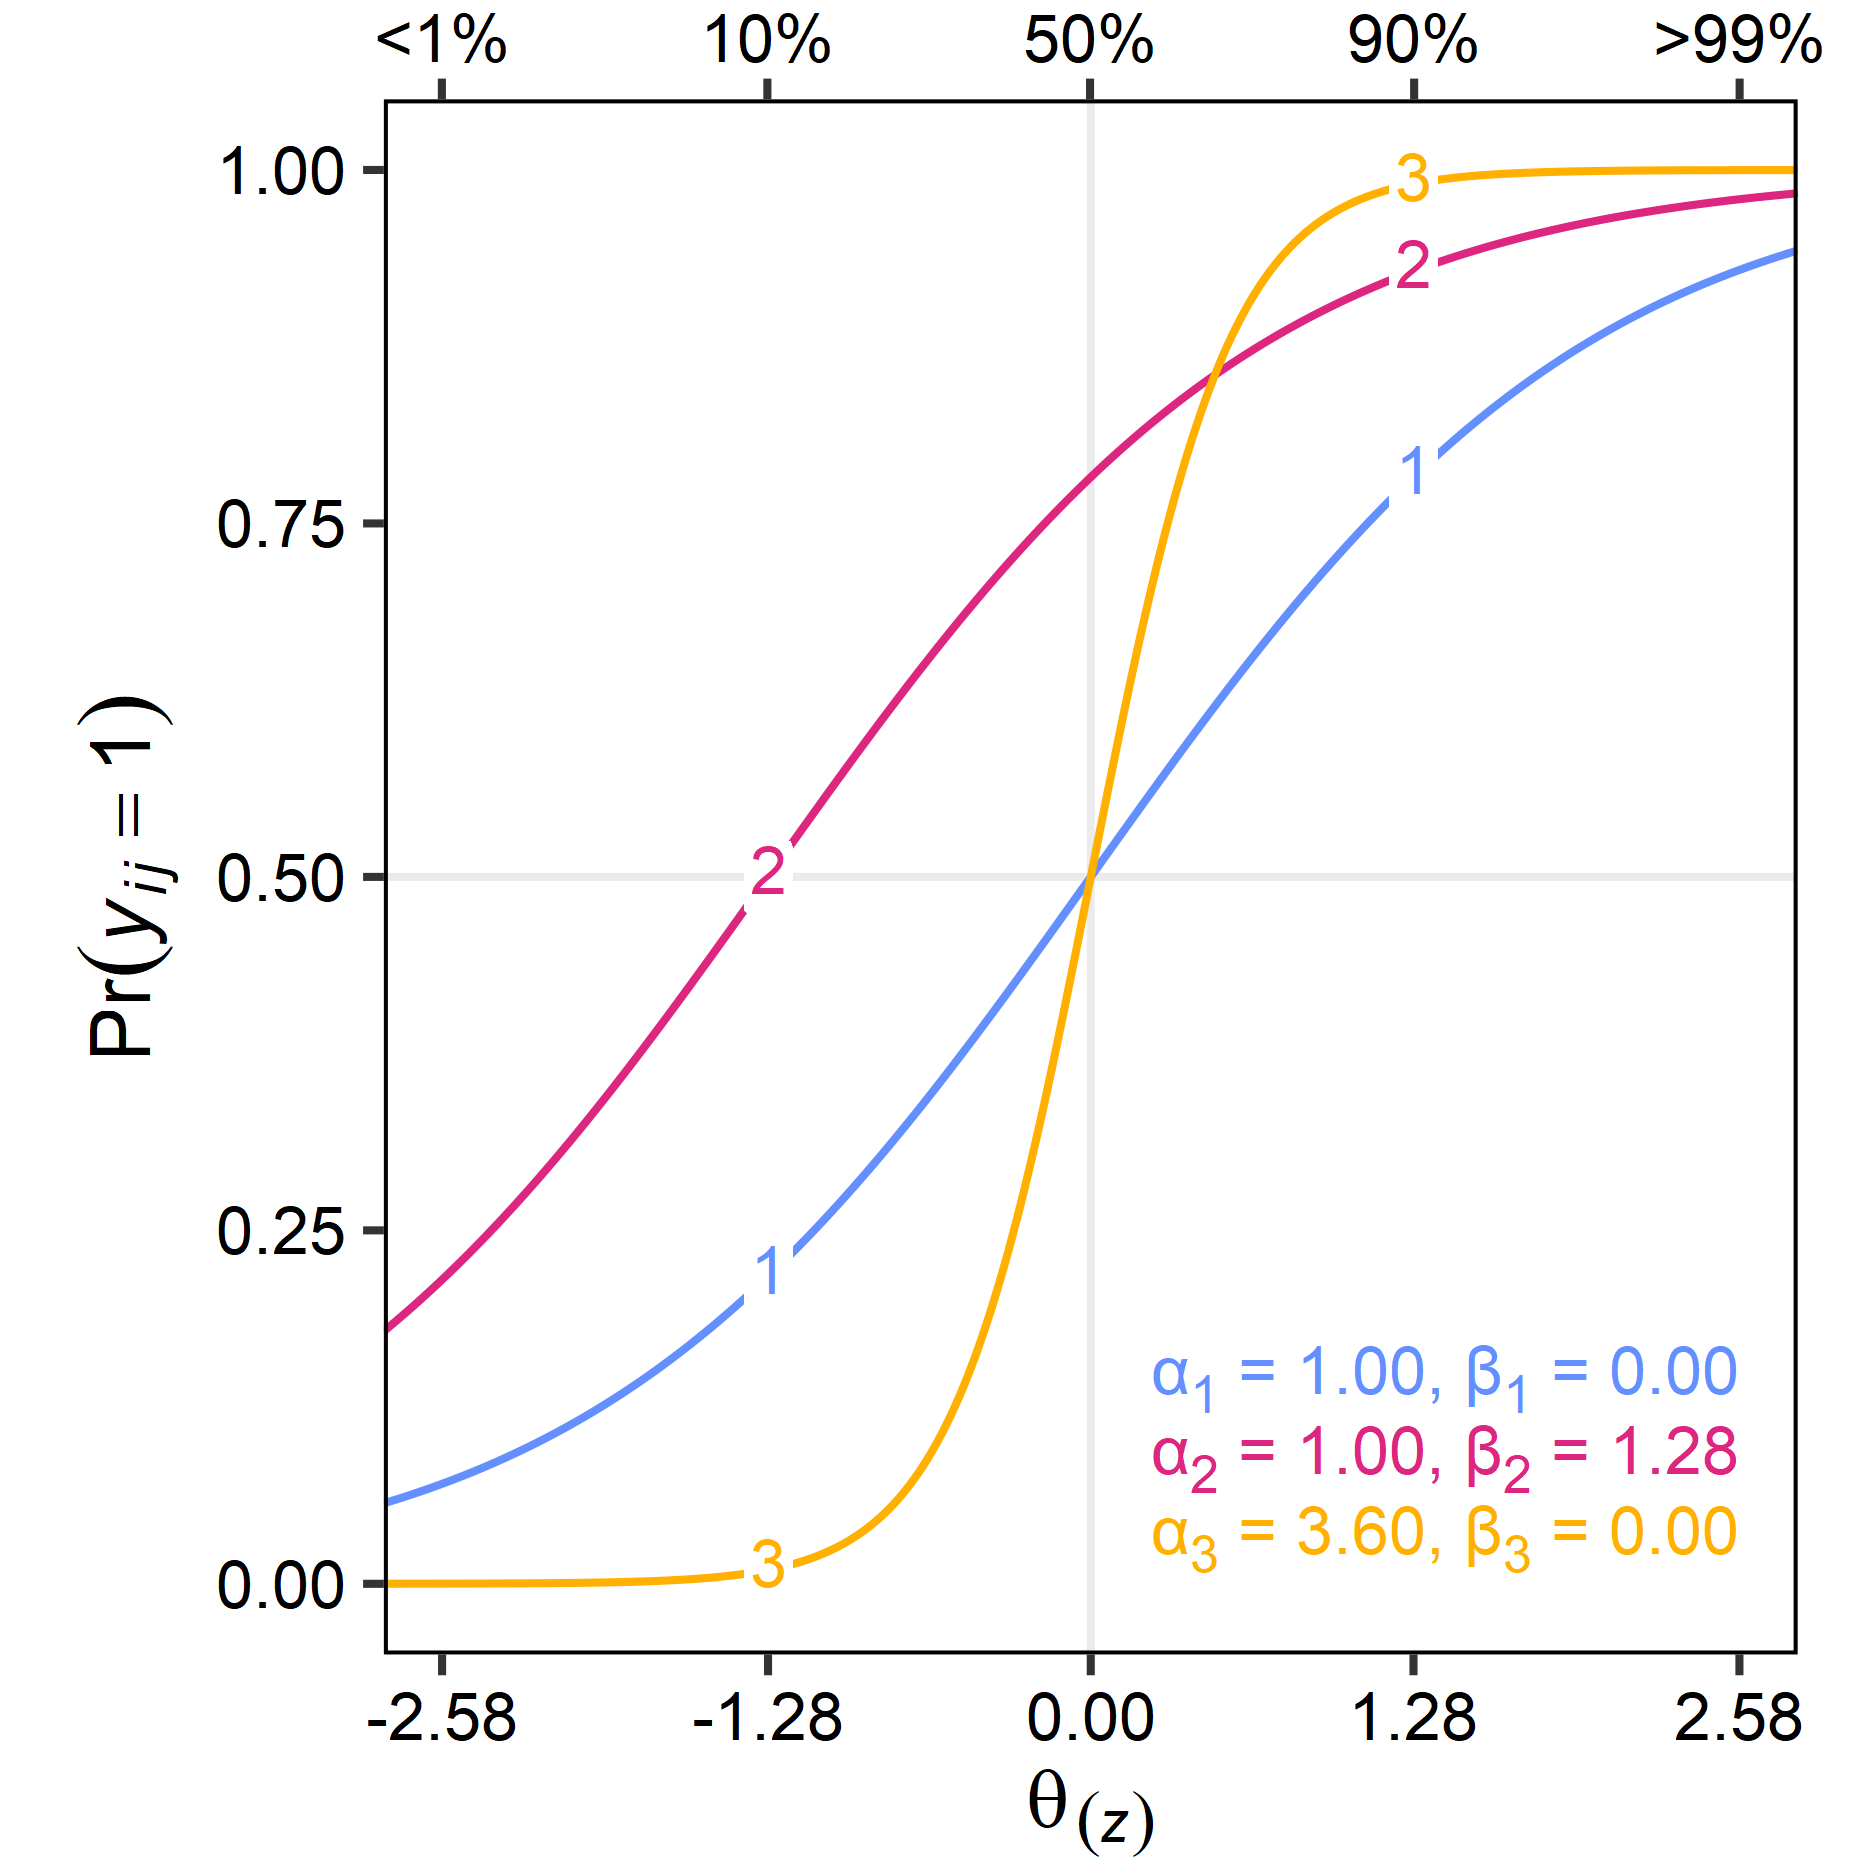
\includegraphics[scale=1]{../Scale Development/figures/figure-1.png}
\caption*{\textit{Note.} $\theta_{(z)}$ follows a standard normal distribution and is shown as both $z$-scores (bottom) and percentiles (top).}
\label{fig:f1}
\end{figure}

In this research, item response theory serves two purposes. First, it
provides a statistical framework for scale development. In Studies 1 and
2, we select the most discriminating and informative actions to build an
instrument for capturing double standards in judging collective action.
Second, it provides a formal and statistical definition of double
standards in judging collective action as respondents being more
accepting of the same protest actions depending on who the protesters
are and what they are protesting. In Experiments 1--3, we operationalize
double standards as differences in \(\theta_{(z)}\) which, as
\(\theta_{(z)}\) is \(z\)-standardized, correspond to Cohen's \(d\)
effect sizes.

\hypertarget{purpose-of-the-present-research}{%
\subsection{Purpose of the Present
Research}\label{purpose-of-the-present-research}}

Five studies (total \(N = 2,979\)) investigate double standards in
judging collective actions---that is, whether observers judge the same
controversial protest actions to be more acceptable depending on who the
protesters are and what they are protesting.

Our first purpose is to develop an instrument to measure where people
draw the line between normative (acceptable) and non-normative
(unacceptable) forms of collective action. In Study 1, we ask
participants to generate more and less extreme protest actions and
compile a pool of protest actions for scale development. In Study 2, we
ask participants to rate how acceptable they consider each of those
protest actions to be and use item response theory to select the most
discriminating and informative protest actions for our instrument. In so
doing, we build an instrument that enables both present and future
research to capture double standards in judging collective action.

Our second purpose is to investigate potential double standards in
judging collective action. Three preregistered experiments used the
newly developed instrument to compare how acceptable participants
controversial protest actions in different conditions.

By varying the participants' and the protesters' group memberships, we
test for ingroup bias in terms of social class when judging protests for
workers' rights (Experiment 1), in terms of race when judging protests
for and against defunding the police (Experiment 2), and in terms of
gender when judging protests for and against restricting abortion
(Experiment 3). In this way, we test the hypothesis that people will
judge the same protest actions as more acceptable if the protesters are
ingroup members or the cause of the protest aligns with the ingroup's
interests.

By varying the protesters' causes, we test whether participants who
identify as left-wing/liberal (Experiments 1--3) and reject
system-justifying beliefs (Experiments 1--2) judge the same protest
actions to be more acceptable when the protesters' cause is progressive
and system challenging (for workers' rights, for defunding the police,
against restricting abortion). Likewise, we test whether participants
who identify as right-wing/conservative and endorse system-justifying
beliefs judge the same protest actions to be more acceptable when the
protesters' cause is conservative and system defending (against
defunding the police, against restricting abortion). In this way, we
test the hypothesis that people will judge the same protest actions as
more acceptable if the cause of the protest aligns with their own
ideological positions.

\hypertarget{scale-development}{%
\section{Scale Development}\label{scale-development}}

In two studies, we developed an instrument of 25 protest actions to
capture double standards in judging collective action.

In Study 1, we compiled protest actions from participants' responses and
other sources. We recruited 60 participants from the Prolific subject
pool, all of whom were citizens of the UK or the US. To increase the
socioeconomic diversity of our sample, we recruited 30 non-students
without a university degree, 15 non-students with a university degree,
and 15 current university students. Participants first read an
accessible definition of what a social group is and that collective
action is any action group members take to promote the interests of
their social group.

\begin{quote}
Society is not only made up of individuals, but consists of `social
groups' to which these individuals belong. Each person lives in a place,
has a job (or not) at an organisation, is a fan of a specific sports
club, has a religion, or belongs to any number of other such groups.
Individuals often act in ways to promote the interests of the social
groups to which they belong.
\end{quote}

\noindent Participants were then asked to name between five and ten
actions that fit that definition. Participants were encouraged to think
of actions that varied in how acceptable they were in their opinion. We
recoded responses into a smaller set of unique actions, which we
supplemented with protest actions from the psychological and political
science literature (e.g., Sharp, 1973). This process resulted in 72
actions that varied in how acceptable we would expect them to be. For
details, see Supplemental Online Material (SOM).

In Study 2, we measured how acceptable participants judged the actions
from Study 1 to be and applied item response theory to develop an
instrument to capture double standards in judging collective action. We
recruited 158 participants (\(\textit{Mdn} = 30\) years, age range:
18--68 years; 103 women, 52 men, 2 other, 1 prefer not to say) from the
Prolific subject pool, all of whom were citizens of the UK or the US. To
increase the socioeconomic diversity of our sample, we recruited 80
non-students without a university degree, 37 non-students with a
university degree, and 41 current university students. We excluded 15
participants who failed an attention check, leaving a final sample of
143 participants for our analyses.

\begin{figure*}[!t]
\centering
\caption{Examples of protest actions rated in Study 2}
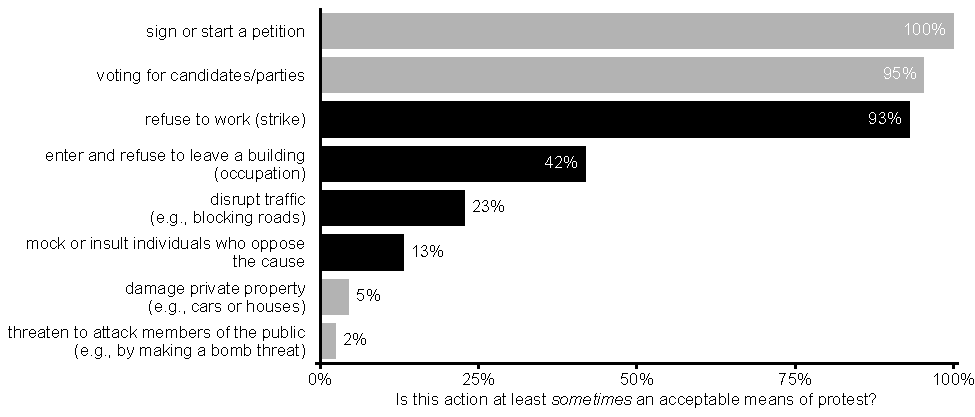
\includegraphics[scale=1]{../Scale Development/figures/figure-2}
\caption*{\textit{Note.} Percentages reflect the proportion of participants who thought that an action was \textit{sometimes}, \textit{often}, or \textit{always} an acceptable means to a advance a cause. Darker bars mark actions that were included in the final scale.}
\label{fig:f2}
\end{figure*}

Participants again read an accessible definition of collective action.
Participants were then asked to think of different causes and
circumstances and to rate how often a given action would be an
acceptable means for a group to advance one of these causes (1 =
\emph{never}, 2 = \emph{rarely}, 3 = \emph{sometimes}, 4 = \emph{often},
5 = \emph{always}). In addition, participants rated how disruptive,
violent, and extreme they considered an action to be (1 = \emph{not at
all}, 4 = \emph{very}) and how positive or negative they felt, in
general, about an action (1 = \emph{very positive}, 5 = \emph{very
negative}). Each participant rated 20 of the 72 actions from Study 1 so
that each action was rated by 29--53 participants.

We estimated a graded response model (Bürkner, 2021; Samejima,
1997)---an item response theory model for ordinal response
variables---for participants' ratings of how often an action would be an
acceptable form of collective action.\footnote{Ratings of how often a
  given action would be an acceptable form of collective action were
  strongly and negatively correlated with how disruptive, violent, and
  extreme participants considered the action to be and how negative they
  felt about it (Table S3).} Based on the results, we selected the 25
most discriminating, informative, and relevant protest actions to form
an instrument for measuring double standards in judging collective
action in Experiments 1--3. We selected controversial, and thus
diagnostic, actions (e.g., disrupting traffic) over actions that almost
all respondents considered acceptable (e.g., signing petitions) or
unacceptable (e.g., political violence; Figure \ref{fig:f2}). For
detailed ratings and results, see SOM.

\hypertarget{experiment-1}{%
\section{Experiment 1}\label{experiment-1}}

In Experiment 1, we used the newly developed instrument to test for
double standards in judging collective action for workers' rights in the
United Kingdom. That is, we tested whether people with either
working-class or professional jobs applied different standards when
judging collective action taken by people with either working-class or
middle-class jobs to protest against a fictitious government bill
threatening their group's rights.

By varying the participants' and the protesters' group memberships, we
tested the preregistered hypothesis that participants would judge the
same protest actions as more acceptable if the protesters were ingroup
members protesting for the ingroup's rights than if they were outgroup
members protesting for the outgroup's rights. By comparing reactions to
working-class and middle-class protesters, we further tested how
observers judge collective action by lower-status (i.e.~working-class)
and higher-status (middle-class) group members.\footnote{For Experiments
  1 and 2, we had preregistered the additional hypotheses that all
  participants would judge the same actions as more acceptable when the
  protesters were from the higher-status group rather than the
  lower-status group (Experiment 1) and when the goal of the protest was
  to support rather than challenge the system (Experiment 2). These
  hypotheses reflected the assumption that the motivation to justify the
  system was, to some extent, universal. With hindsight, we no longer
  think that this assumption is tenable and, therefore, omit the
  hypotheses based on it from the revised manuscript. We still report
  the same preregistered analyses and their results.} In
non-preregistered analyses, we tested whether participants would judge
the same protest actions as more or less acceptable depending on their
own ideological positions in terms of political orientation,
system-justifying beliefs, and social dominance orientation.\footnote{In
  Experiment 1, we explored a broader range of operationalizations of
  political ideology, including social dominance orientation, than in
  the other experiments.} In this way, Experiment 1 provided a first
test of the hypothesized class- and ideology-based double standards in
judging collective action.

\hypertarget{method}{%
\subsection{Method}\label{method}}

\hypertarget{transparency-and-openness}{%
\subsubsection{Transparency and
Openness}\label{transparency-and-openness}}

We preregistered the sample size as well as all hypotheses,
inclusion/exclusion criteria, measures, and manipulations
(\url{https://osf.io/24wrx/?view_only=8560eb60286149498f8da48bc9f9d99b}).
We made all materials, data, and analysis scripts available online
(\url{https://osf.io/d3yev/?view_only=40782034017c40f0bcecb1cc87760b62}).
We followed sample size recommendations for item response theory models
(DeMars, 2010, p. 36), planning to recruit 500 participants.

\hypertarget{study-design}{%
\subsubsection{Study Design}\label{study-design}}

We used a 2 (quasi-experimental: higher-status/lower-status
participants) \(\times\) 2 (experimental: higher-status/lower-status
protesters) between-subjects design to test our hypotheses.

\hypertarget{participants}{%
\subsubsection{Participants}\label{participants}}

We recruited 515 participants from the Prolific subject pool who were UK
citizens, 25 years old or older, and not current students.\footnote{We
  had preregistered a sample of 500 participants, before exclusions, but
  included another 15 participants who completed the study without
  returning an approval code to the Prolific platform. Participants
  received, on average, \pounds 9.00 (\$10.93) per hour of
  participation.} As preregistered, we excluded 71 participants who
failed an attention check. This resulted in a final sample of 443
participants (\(\textit{Mdn} = 41\) years, age range: 25--76 years; 272
women, 171 men, 1 non-binary). Of these, 210 participants considered
their past, current, or future jobs to be working-class jobs.
Participants in this lower-status group did not have a university degree
and placed themselves on the bottom three ranks of the subjective
socioeconomic status ladder. Another 233 participants considered their
past, current, or future jobs to be middle-class/professional jobs.
Participants in this higher-status group had at least an undergraduate
degree and placed themselves on the top four ranks of the subjective
socioeconomic status ladder. On average, participants tended to describe
their political orientation as somewhat left-wing
(\(\textit{M} = 3.54\), \(\textit{SD} = 1.31\)) with \(36\%\) and
\(20\%\) describing their political orientation as, respectively, at
least somewhat left-wing and right-wing.

\hypertarget{procedure}{%
\subsubsection{Procedure}\label{procedure}}

We used a screening survey to recruit participants who satisfied our
preregistered inclusion criteria for the lower-status and higher-status
groups. For the lower-status group, we recruited participants who did
not have a university degree and placed themselves on the bottom three
ranks of a subjective socioeconomic status ladder. For the higher-status
group, we recruited participants who had at least an undergraduate
degree and placed themselves on the top four ranks of the subjective
socioeconomic status ladder.

In the screening survey, participants read an accessible definition of
what working-class and middle-class/professional jobs are (for details,
see SOM). Participants then answered, among other questions, whether
they considered their current job---or the jobs they had had in the past
or expected to have in the future---to be a working-class job or a
middle-class/professional job. As preregistered, we excluded
participants from the lower-status group who did not respond
``working-class job'' and participants from the higher-status group who
did not respond ``middle-class/professional job''.

We recruited 500 participants from the remaining participants, 250 from
the lower-status group and 250 from the higher-status group.
Participants were randomly assigned to read a vignette about a
government bill affecting either people in working-class jobs
(lower-status protesters) or people in professional jobs (higher-status
protesters). Participants in both conditions were instructed to
carefully read the vignette and to try to imagine what it would be like
if this situation was real. Participants in the lower-status protesters
condition read the following introduction:

\begin{quote}
The government, though not necessarily the current government, is going
to introduce a bill that will mostly affect people in working-class
jobs. Working-class jobs, in this case, are jobs done by skilled,
semi-skilled, unskilled manual workers or by casual workers. These are
jobs that do not usually require a university degree. Other jobs are
unlikely to be affected.
\end{quote}

\noindent Participants in the higher-status protesters condition instead
read the following introduction:

\begin{quote}
The government, though not necessarily the current government, is going
to introduce a bill that will mostly affect people in professional jobs.
Professional jobs are administrative, managerial, or other jobs that
usually require a university degree. Other jobs are unlikely to be
affected.
\end{quote}

\noindent Participants in both conditions then read an almost
identically worded paragraph:

\begin{quote}
This government measure would make it easier for companies to hire
workers during economic growth and to lay off workers during an economic
crisis. As a consequence, companies would be able to fire employees with
little notice and without giving a reason. Trade unions are opposed to
the measure. They argue that the bill would compromise job security, and
prevent employees from challenging harassment or other abuse without the
fear of being fired. People in {[}working-class/professional{]} jobs are
particularly at risk, and there is a rise in tension and outrage among
them.
\end{quote}

On the next pages, participants completed all remaining measures. On the
final page, we asked participants to recall who the people most affected
by the fictitious government bill were. As preregistered, we excluded
all participants whose response did not qualitatively match their
experimental condition.

\hypertarget{measures}{%
\subsubsection{Measures}\label{measures}}

We measured the outcome variable by asking participants to decide, for
each of 25 protest actions presented in a randomized order, whether they
thought this action was ``an acceptable means for people in
{[}working-class/professional{]} jobs to protest against the government
bill'' (1 = \emph{yes}, 0 = \emph{no}; see Table A1).

We assessed reactions to the vignette by asking participants how
outraged they would be if the government were to introduce this bill in
real life, to what extent it would affect them personally, and to what
extent it would affect people like them (1 = \emph{not at all}, 7 =
\emph{very much}). We also asked participants to what extent they
identified with people with the kinds of jobs most affected by the
proposed bill (1 = \emph{not at all}, 7 = \emph{very much}) and how
often, if at all, they had participated in protest actions such as the
ones we asked about (1 = \emph{never}, 5 = \emph{very often}).

We measured social dominance orientation with the eight-item
\(\text{SDO}_{7(s)}\) scale (Ho et al., 2015), for example, ``it is
unjust to try to make groups equal'' (1 = \emph{strongly oppose}, 7 =
\emph{strongly favour}; McDonald's \(\omega = .89\)). A confirmatory
factor analysis model in which all items loaded onto a single factor
showed acceptable fit,
\(\chi^2 (20) = 108.69; \text{CFI} = 0.92; \text{TLI} = 0.88; \text{RMSEA} = 0.11, [0.09, 0.14]\).

We measured system-justifying beliefs with eight items (adapted from Kay
\& Jost, 2003), for example, ``in general, I find society to be fair''
(1 = \emph{strongly disagree}, 7 = \emph{strongly agree}; McDonald's
\(\omega = .89\)). A confirmatory factor analysis model in which all
items loaded onto a single factor showed acceptable fit,
\(\chi^2 (20) = 77.37; \text{CFI} = 0.94; \text{TLI} = 0.92; \text{RMSEA} = 0.09, [0.07, 0.12]\).

In the screening survey, we recorded participants' gender, age,
nationality, student status, and employment status. We also included two
three-item scales measuring social identification with people in
working-class and middle-class/professional jobs (adapted from Becker et
al., 2011) and a one-item semantic differential scale measuring
political orientation (``People often describe their political
orientation as left-wing or right-wing. On a scale from left to right,
where would you position yourself?''; 1 = \emph{left}, 7 =
\emph{right}).

\hypertarget{results}{%
\subsection{Results}\label{results}}

\begin{figure*}[!t]
\centering
\caption{Results from the preregistered (\textbf{A}) and non-preregistered (\textbf{B}) analyses for Experiment 1}
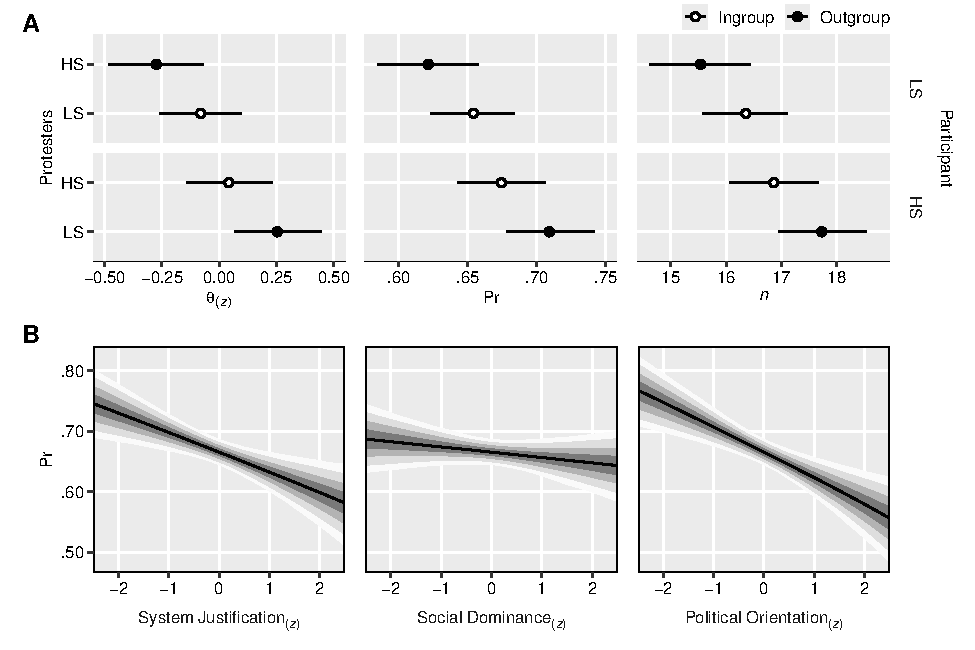
\includegraphics[scale=1]{../Experiment 1/figures/figure-3}
\caption*{\textit{Note.} HS = Higher Status, LS = Lower Status. $\theta_{(z)}$ is the \textit{z}-standardized tendency to consider more controversial actions acceptable means of protest. (\textbf{A}) $p$ and $n$ are, respectively, the predicted proportion and number of actions a participant would consider acceptable means of protest in each condition. Bars enclose the 95\% most plausible estimates. (\textbf{B}) Ribbons enclose, from the darkest to the lightest shade, the 50\%, 80\%, 95\%, and 99\% most plausible estimates.}
\label{fig:f3}
\end{figure*}

\hypertarget{reactions-to-the-manipulation}{%
\subsubsection{Reactions to the
Manipulation}\label{reactions-to-the-manipulation}}

Participants with professional jobs thought that they would be more
outraged if the government were to introduce a bill affecting people
with similar jobs (\(M = 6.00, SD = 1.05\)) than by a bill affecting
people with working-class jobs (\(M = 5.38, SD = 1.28\); Cohen's
\(d = 0.50\)). Conversely, participants with working-class jobs thought
that they would be more outraged by a bill affecting people in similar
jobs (\(M = 6.26, SD = 1.05\)) than by a bill affecting people in
professional jobs (\(M = 5.61, SD = 1.47\); \(d = 0.52\)). Participants
thought that a bill affecting people with similar jobs would affect them
personally (\(d = 1.14\)) and people like them (\(d = 1.33\)) more than
a bill affecting people with other jobs. Participants identified to a
greater extent with people in similar jobs (\(M = 6.21, SD = 1.12\))
than with people in other jobs (\(M = 4.06, SD = 1.65\); \(d = 1.22\)).
Overall, participants' reactions suggested that the experimental design
worked as intended and that participants in the lower-status and
higher-status groups understood the vignette in ingroup--outgroup terms.

\hypertarget{preregistered-analyses}{%
\subsubsection{Preregistered Analyses}\label{preregistered-analyses}}

To test our hypotheses, we estimated a two-parameter logistic item
response theory model (Bürkner, 2021) with participants' responses to
the question whether they thought each action was an acceptable means of
protest as the outcome variable. For each action \(i\), the model
estimated how acceptable (\(\beta_i\)) and discriminating (\(\alpha_i\))
that protest action was. For each participant \(j\), the model estimated
their unique propensity to consider protest actions acceptable
(\(\theta_j\)). In addition, the model estimated how accepting
participants were of controversial protest actions as a function of
three dummy-coded variables that encoded the group status of the
protesters and the participant.

We estimated this model in CmdStan (Gabry \& Cesnovar, 2021; Stan
Development Team, 2021) using Bayesian statistical methods. Bayesian
inference involves choosing a likelihood function and prior
distributions. A likelihood function links the observed data to the
model parameters and states how likely the observed data are given
different values of said model parameters. Prior distributions state how
plausible different values of said model parameters are before
considering the observed data. Bayesian inference applies Bayes' theorem
to update prior distributions in light of the observed data to produce
posterior distributions. In contrast to \(p\)-values and confidence
intervals, posterior distributions have a straight-forward
interpretation as stating how plausible different values of the model
parameters are given the observed data.

Our model derived the likelihood of participants' responses from a
Bernoulli likelihood function with a logistic regression equation
linking the two item parameters (\(\alpha_i\), \(\beta_i\)), the one
participant parameter (\(\theta_j\)), and the three regression
coefficients to the observed data. To identify the model, we constrained
\(\theta_j\) to have a mean of zero and constrained \(\alpha_i\) to have
a fixed mean and to be non-negative. We used partial pooling to estimate
\(\alpha_i\), \(\beta_i\), and \(\theta_j\). Our model assigned weakly
informative prior distributions (Gelman et al., 2017) to all model
parameters.\footnote{Our model assigned \(\text{Half-Cauchy} (0, 3)\)
  prior distributions to the standard deviations of \(\alpha_i\),
  \(\beta_i\), and \(\theta_j\) and \(\text{Normal} (0, 3)\) prior
  distributions to all other model parameters.} We report point
estimates, based on the median of posterior samples, and uncertainty
intervals, based on the quantiles of posterior samples, that enclose the
95\% most plausible estimates.

Figure \ref{fig:f3} (A) shows estimates for each combination of the
protesters' and the participants' group membership. Overall, we found
that participants' responses depended on both the protesters' and the
participants' group status---but not in the directions predicted by our
hypotheses. Contradicting our hypothesis, participants did not consider
protest actions performed by their ingroup to be more acceptable, on
average, than the same actions performed by the relevant outgroup
(Cohen's \(d = 0.00, [-0.20, 0.20]\)). Instead, we found that
participants from higher-status backgrounds considered protest actions
performed by both lower-status (\(d = 0.34, [0.07, 0.59\){]}) and
higher-status (\(d = 0.33, [0.03, 0.63]\)) protesters to be, on average,
more acceptable than participants from lower-status backgrounds. All
participants considered protest actions performed by higher-status
protesters to be less acceptable, on average, than the same actions
performed by lower-status protesters (\(d = -0.20, [-0.40, -0.00]\)).

\hypertarget{non-preregistered-analyses}{%
\subsubsection{Non-Preregistered
Analyses}\label{non-preregistered-analyses}}

We explored to what extent participants' ideological orientations
influenced how acceptable they considered various protest actions to be.
To that end, we estimated another two-parameter logistic item response
model that estimated participants' responses as a function of the
participant's and the protesters' group status and of the participants'
political orientation, social dominance orientation, and
system-justifying beliefs. We used factor scores to quantify social
dominance orientation and system-justifying beliefs and standardized all
new predictor variables. We report standardized regression coefficients
that quantify by how many standard deviations a participant's propensity
to consider more collective actions acceptable increases for each
additional standard deviation of the predictor variable.

Figure \ref{fig:f3} shows (B) the \(z\)-standardized propensity to
consider more controversial protest actions acceptable as a function of
the three ideological orientation variables. We found that participants
who reported a more right-wing political orientation
(\(\beta_{xy} = -0.25, [-0.37, -0.15]\)) and who expressed more
agreement with system-justifying beliefs
(\(\beta_{xy} = -0.20, [-0.30, -0.10]\)) tended to find fewer collective
actions to be acceptable. In contrast, we found that, after controlling
for the other two variables, social dominance orientation was not
associated with participants' judgments about how acceptable various
collective actions are (\(\beta_{xy} = -0.05, [-0.15, 0.05]\)). Overall,
these findings suggest that people who are right-wing and endorse
system-justifying beliefs tend to find various collective actions to be
less acceptable than people who are left-wing and do not endorse
system-justifying beliefs.\footnote{We ran additional analyses to
  explore how these associations differed across experimental
  conditions. We found uncertainty intervals for these associations to
  overlap across conditions, suggesting that we did not have enough data
  to differentiate these varying effects.}

\hypertarget{discussion}{%
\subsection{Discussion}\label{discussion}}

Experiment 1 provided a first test of the hypothesized group-based
double standards in judging collective action. That is, we tested
whether, as hypothesized, participants would judge the same protest
actions as more acceptable if the protesters were ingroup members
protesting for the ingroup's rights. We found that participants'
responses depended on both the participants' and the protesters' group
memberships---but not in the hypothesized directions. Both lower-status
and higher-status participants tended to find the same protest actions
more acceptable when lower-status protesters protested a bill
threatening their rights. In non-preregistered analyses, we found
evidence for ideology-based double standards as people who were
right-wing and endorsed system-justifying beliefs tended to find all
protest actions to be less acceptable.

Experiment 1 did not, however, provide a conclusive test of our
hypotheses. First, by focusing on fictitious government bills, we might
have chosen a scenario too far removed from current affairs to evoke
strong ingroup bias in participants' judgments of protest actions. That
said, participants' reactions to the experimental manipulation suggested
that it evoked outrage and was understood in ingroup--outgroup terms.
Second, by focusing on collective action to defend workers' rights, we
studied reactions to collective action for a progressive cause. To test
for ideology-based double standards, we needed to vary the protesters'
cause to compare reactions to both progressive and conservative causes.
Experiment 2 addressed those limitations by focusing on a scenario we
expected to evoke stronger responses from participants and by examining
reactions to both system-challenging and system-defending collective
action.

\hypertarget{experiment-2}{%
\section{Experiment 2}\label{experiment-2}}

In Experiment 2, we investigated potential double standards in judging
collective action for or against defunding the police in the United
States. That is, we tested whether Black and White Americans applied
different standards when judging collective action taken by either Black
or White protesters to protest either for or against police divestment
as a possible solution to racist police violence. We conducted this
study in January 2021, a time when, after months of unprecedented
protests for racial justice, most Americans could be expected to be
aware of, and have formed an opinion on, the Black Lives Matter movement
(Leach \& Allen, 2017; Leach \& Teixeira, 2022). We focused on defunding
the police as this position remained controversial among both Black and
White Americans even as they broadly agreed on the need for police
reform.\footnote{In December 2020, only 34\% of Black Americans and 18\%
  of White Americans supported defunding the police while majorities of
  Black and White Americans supported police reforms such as eliminating
  qualified immunity (50\% and 57\%) or banning chokeholds (79\% and
  61\%, YouGov, 2020).}

By varying the participants' and the protesters' group memberships, we
tested the preregistered hypothesis that participants would judge the
same protest actions as more acceptable if the protesters were ingroup
members. By assuming that defunding the police aligns more closely with
the interests of Black than White Americans, we tested the preregistered
hypothesis that participants would judge the same protest actions as
more acceptable if the cause of the protest aligned with their ingroup's
interests. By varying whether the protesters protested for or against
defunding the police, we tested the preregistered hypotheses that
participants would judge the same protest actions as more acceptable if
they endorsed system-justifying beliefs and the protest supported the
system or if they rejected system-justifying beliefs and the protest
challenged the system. In this way, Experiment 2 provided a complete
test of the hypothesized race- and ideology-based double standards in
judging collective action. In addition, we tested the simpler,
alternative hypothesis that participants, in general, would judge the
same protest actions as more acceptable if they supported the
protesters' cause.

\hypertarget{method-1}{%
\subsection{Method}\label{method-1}}

\hypertarget{transparency-and-openness-1}{%
\subsubsection{Transparency and
Openness}\label{transparency-and-openness-1}}

We preregistered the sample size as well as all hypotheses,
inclusion/exclusion criteria, measures, and manipulations
(\url{https://osf.io/skxjt/?view_only=d8ce44a700884b5ab36b64ef08f833a1}).
We made all materials, data, and analysis scripts available online
(\url{https://osf.io/d3yev/?view_only=40782034017c40f0bcecb1cc87760b62}).
As reported in the preregistration, we ran simulations, using data from
Experiment 1, to determine that a sample size of \(N = 1,600\)
(\(n = 200\) per condition) was sufficient to detect even small
differences between conditions (\(0.09 < \text{Cohen's}~d < 0.16\)).

\hypertarget{study-design-1}{%
\subsubsection{Study Design}\label{study-design-1}}

We used a 2 (quasi-experimental: Black/White participants) \(\times\) 2
(experimental: Black/White protesters) \(\times\) 2 (experimental:
for/against defunding the police) between-subjects design to test our
hypotheses.

\hypertarget{participants-1}{%
\subsubsection{Participants}\label{participants-1}}

We recruited 1,773 Black and White American participants from the
Prolific subject pool who were 18 years old or older, lived in the US,
and were US citizens.\footnote{Data were collected between January 15
  and 28, 2021. Participants received, on average, \$12.89 per hour of
  participation.} As preregistered, we excluded 173 participants who
failed at least one of three attention checks or who reported a
different ethnic background than they had reported in the Prolific
prescreening questionnaire. This resulted in a final sample of 1,600
participants (\(\textit{Mdn} = 31\) years, age range: 18--84 years; 864
women, 708 men, 27 sex/gender diverse) of whom 800 identified as Black
and 800 identified as White. On average, participants tended to describe
their political orientation as moderately liberal
(\(\textit{M} = 2.92\), \(\textit{SD} = 1.73\)) with \(63\%\) and
\(16\%\) describing their political orientation as, respectively, at
least somewhat liberal and conservative.

\hypertarget{procedure-1}{%
\subsubsection{Procedure}\label{procedure-1}}

Participants read the following paragraphs:

\begin{quote}
In 2020, police officers killed Breonna Taylor and George Floyd. Many
were outraged that police officers had, once again, killed unarmed Black
Americans. Across the United States, people called for changes to
prevent future police violence.
\end{quote}

\begin{quote}
Some argue that, to end police violence, we should take money away from
police departments. Reducing police funding would mean fewer police
officers on the street. Fewer police officers would mean fewer
opportunities for them to turn violent. Reducing police funding would
also leave more money for other services. Proponents argue for
reallocating police funding to social services, housing, and education.
Doing so would keep communities safer with fewer police officers. We
refer to this position as ``defunding the police''. This position
differs from ``reforming the police'' which might mean increasing police
funding and also differs from ``abolishing the police'' which means
disbanding police departments altogether.
\end{quote}

\noindent Participants were then asked to answer whether the text had
been about ``reforming the police'', ``defunding the police'', or
``abolishing the police''. If they selected the wrong answer, they were
instructed to reread the text and select the right answer. On the next
page, participants stated whether they supported or opposed the proposed
solution.

Participants in the system-challenging protest condition then read a
text about protesters in support of defunding the police:

\begin{quote}
Earlier, you read about defunding the police as a possible solution to
end police violence. Some local residents want to protest for defunding
the police. They argue that reducing police funding would prevent police
violence.
\end{quote}

\noindent Participants in the system-supporting protest condition
instead read about protesters rallying against defunding the police:

\begin{quote}
Some local residents want to protest against defunding the police. They
argue that reducing police funding would mean fewer police officers
serving their community.
\end{quote}

\noindent Participants then read either that ``most of the protesters
are Black'' or that ``most of the protesters are White''. Participants
again had to correctly answer multiple choice questions about the text
(``Are the protesters for or against defunding the police?'', ``Who are
the protesters?'') before being able to proceed.

On the next pages, participants completed all remaining measures. On the
final page, participants responded to three attention checks: ``In this
study, you first read about a proposed solution to police violence. What
was it?'' (\emph{reforming the police}, \emph{defunding the police},
\emph{abolishing the police}); ``In this study, you then read about
protesters. Were these protesters for or against the proposed
solution?'' (\emph{for}, \emph{against}); and ``Were most of the
protesters Black or White?'' (\emph{Black}, \emph{White}). As
preregistered, we excluded participants who gave an answer inconsistent
with their assigned experimental condition.

\hypertarget{measures-1}{%
\subsubsection{Measures}\label{measures-1}}

We measured the outcome variable by asking participants to think about
the protesters they had read about and to decide, for each of 25 protest
actions presented in a randomized order, whether they thought this
action was ``an acceptable means for them to protest {[}for/against{]}
defunding the police'' (1 = \emph{yes}, 0 = \emph{no}). We replaced some
actions from Experiment 1 because they either did not fit the study
context or had been considered acceptable by almost all participants
(see Table B1).

We measured system-justifying beliefs with eight items (adapted from Kay
\& Jost, 2003), for example, ``in general, I find society to be fair''
(1 = \emph{strongly disagree}, 7 = \emph{strongly agree}; McDonald's
\(\omega = .91\)). A confirmatory factor analysis model in which all
items loaded onto a single factor showed acceptable fit,
\(\chi^2 (28) = 4309.15; \text{CFI} = 0.95; \text{TLI} = 0.93; \text{RMSEA} = 0.11, [0.10, 0.12]\).

We measured support for defunding the police with one item: ``Do you
support or oppose defunding the police?'' (1 = \emph{strongly oppose}, 5
= \emph{strongly support}).

We included additional measures to describe the sample, to describe
reactions to the manipulation, or to use in non-preregistered analyses.
In addition to demographic questions, we asked participants how outraged
they were about recent incidents of police violence against Black
Americans, to what extent they identifed with the protesters described
in the study, and to what extent they identifed with their racial
ingroup (1 = \emph{not at all}, 7 = \emph{very much}). We also asked how
often, if at all, participants had participated in protest actions such
as the ones we had asked about (1 = \emph{never}, 5 = \emph{very often})
and whether they had participated in protests for reforming, defunding
or abolishing the police; against reforming, defunding or abolishing the
police; or in neither. We measured political orientation with a one-item
semantic differential scale: ``People often describe their political
orientation as liberal or conservative. On a scale from liberal to
conservative, where would you position yourself?'' (1 = \emph{liberal},
7 = \emph{conservative}).

\hypertarget{results-1}{%
\subsection{Results}\label{results-1}}

\begin{figure*}[!t]
\centering
\caption{Results from the preregistered analyses for Experiment 2}
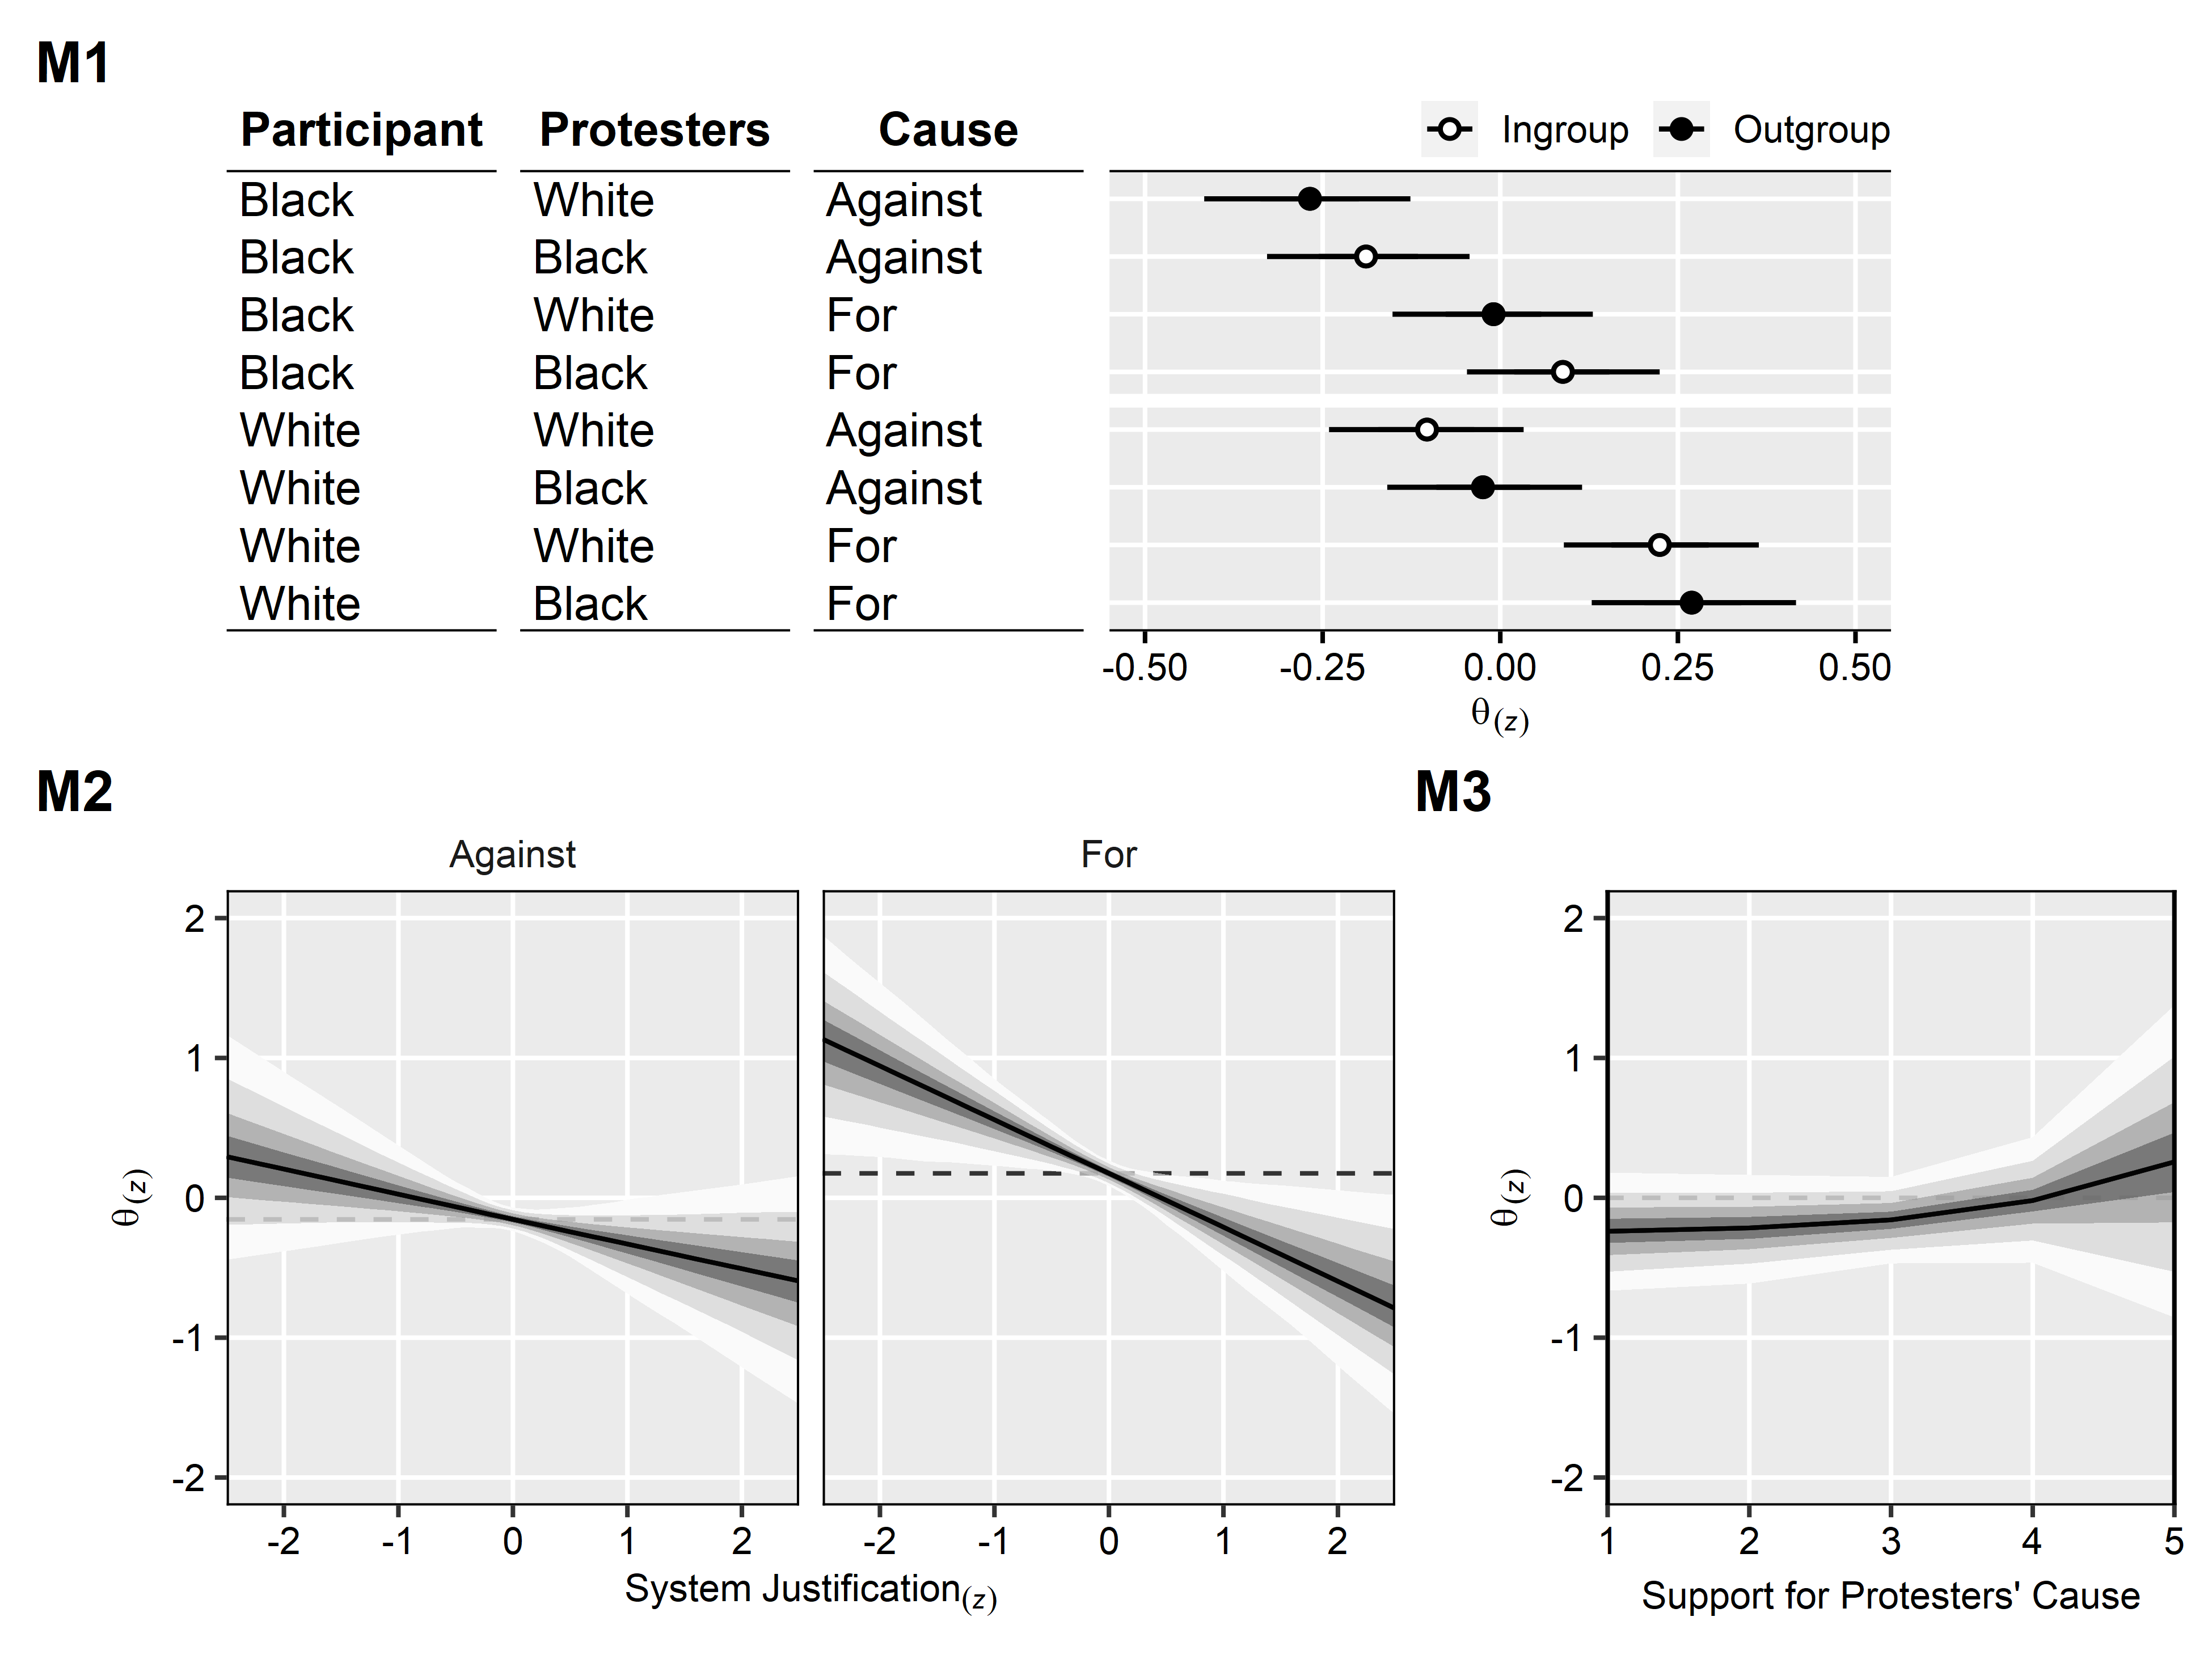
\includegraphics[scale=1]{../Experiment 2/figures/figure-4}
\caption*{\textit{Note.} Against = Protesters oppose defunding the police. For = Protesters support defunding the police. $\theta_{(z)}$ is the \textit{z}-standardized tendency to consider more controversial actions acceptable means of protest. Ribbons enclose, from the darkest to the lightest shade, the 50\%, 80\%, 95\%, and 99\% most plausible estimates.}
\label{fig:f4}
\end{figure*}

\begin{figure*}[!t]
\centering
\caption{Predictions from the preregistered (system justification) and non-preregistered (political orientation) analyses for Experiment 2}
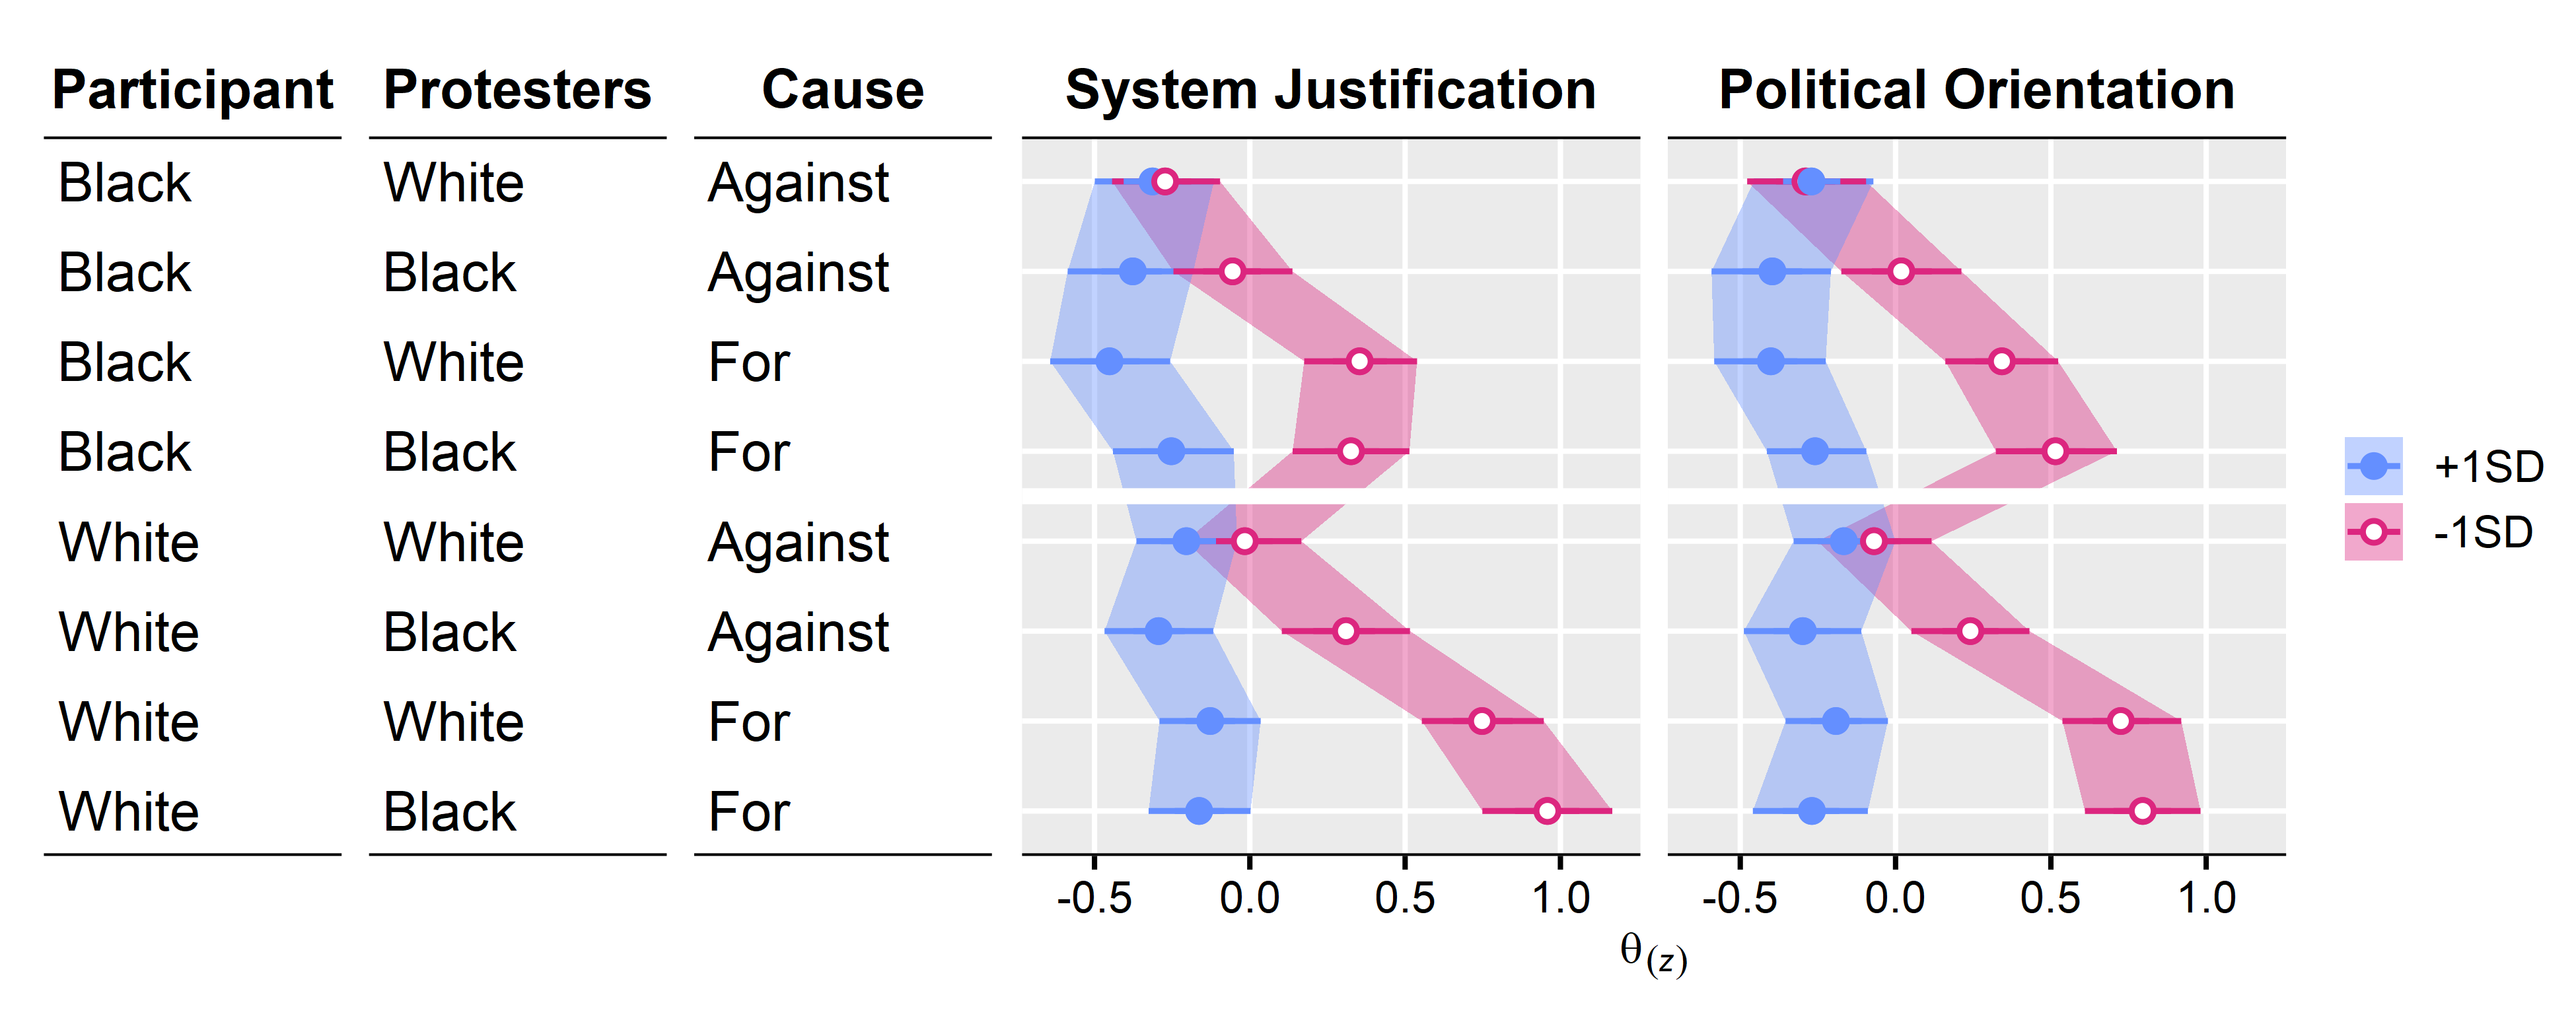
\includegraphics[scale=1]{../Experiment 2/figures/figure-5}
\caption*{\textit{Note.} Against = Protesters oppose defunding the police. For = Protesters support defunding the police. $\theta_{(z)}$ is the \textit{z}-standardized tendency to consider more controversial actions acceptable means of protest.}
\label{fig:f5}
\end{figure*}

\hypertarget{reactions-to-the-manipulation-1}{%
\subsubsection{Reactions to the
Manipulation}\label{reactions-to-the-manipulation-1}}

As expected, Black participants (\(M = 6.18, \textit{SD} = 1.31\))
reported being more outraged about recent incidents of police violence
than White participants (\(M = 5.56, \textit{SD} = 1.61\); Cohen's
\(d = 0.42\)). Black participants strongly identified with their ingroup
(\(M = 6.46, \textit{SD} = 1.09\)) and, across experimental conditions,
identified more with Black protesters (\(M = 4.66, \textit{SD} = 1.99\))
than with White protesters (\(M = 4.03, \textit{SD} = 2.16\);
\(d = 0.30\)). In contrast, White participants identified less strongly
with their ingroup than Black participants
(\(M = 4.85, \textit{SD} = 1.53\); \(d = 1.21\)) and did not identify
more with White protesters (\(M = 3.58, \textit{SD} = 2.01\)) than with
Black protesters (\(M = 3.81, \textit{SD} = 1.77\); \(d = -0.12\)). Both
White (\(d = 0.67\)) and Black (\(d = 0.53\)) participants tended to
identify more with protesters protesting \emph{for} defunding the
police. On average, participants tended to describe their political
orientation as moderately liberal (\(M = 2.92, \textit{SD} = 1.73\))
but, as expected, were divided in their support for defunding the police
(\(M = 3.37, \textit{SD} = 1.42\)). That is, 56\% supported defunding
the police, 30\% opposed defunding the police, and 14\% remained
undecided.

\hypertarget{preregistered-analyses-1}{%
\subsubsection{Preregistered Analyses}\label{preregistered-analyses-1}}

To test our hypotheses, we estimated a series of two-parameter logistic
item response theory models with participants' responses to the question
whether they thought each action was an acceptable means of protest as
the outcome variable. Our models differed from the models used in
Experiment 1 in two ways. First, we estimated the item parameters
(\(\alpha_i\), \(\beta_i\)) as \emph{correlated} varying effects.
Second, we used varying, rather than fixed, effects to estimate
differences between the eight conditions. This resulted in partial
pooling---condition-wise estimates were shrunk towards each other---and
allowed us to compare conditions without multiple comparison problems
(Gelman et al., 2012). Our models assigned weakly informative prior
distributions to all model parameters.\footnote{Our model assigned
  \(\text{LKJ} (2)\) prior distributions to the Cholesky-transformed
  correlation matrices for varying effects and
  \((\text{Half-})\text{Cauchy} (0, 5)\) prior distributions to all
  other model parameters.} Figure \ref{fig:f4} shows results from three
preregistered models we estimated to test our hypotheses.

Model 1 estimated varying intercepts for the eight conditions to test
whether, as hypothesized, participants' responses depended on their own
group membership, the protesters' group membership, or the protesters'
cause. Contradicting the hypothesized race-based double standards,
participants did not consider protest actions performed by their ingroup
to be more acceptable, on average, than the same actions performed by
the relevant outgroup (\(d = 0.01, [-0.04, 0.06]\)). Likewise,
participants did not consider protest actions for a cause that was
nominally aligned with their ingroup's interests to be more acceptable,
on average, than protest actions for a cause not aligned with their
ingroup's interests (\(d = -0.01, [-0.06, 0.04]\)). Instead, we found
that, on average, White participants considered all protest actions to
be more acceptable than Black participants (\(d = 0.09, [0.04, 0.14]\))
and both Black (\(d = 0.13, [0.06, 0.20]\)) and White
(\(d = 0.16, [0.08, 0.23]\)) participants considered the same actions to
be more acceptable when protests were for, rather than against,
defunding the police. As in Experiment 1, we thus found that
participants' responses depended on both the participants' and the
protesters' group memberships---but not in the directions predicted by
our hypotheses.

Model 2 extended Model 1 by estimating participants' responses as a
function of their \emph{z}-standardized endorsement of system-justifying
beliefs. As preregistered, we modeled this relationship with two fixed
effects, one estimating the effect of system-justifying beliefs on
judgments about system-defending protest actions and one estimating
their effect on judgments about system-challenging protest actions, and
one varying effect estimating its variance across conditions. Supporting
the hypothesized ideology-based double standards, participants who
\emph{rejected} system-justifying beliefs were \emph{more} likely to
consider system-challenging protest actions (for defunding the police)
to be acceptable means of protest (\(\beta_{xy} = 0.38, [0.16, 0.58]\)).
We did not, however, find evidence for the hypothesized ideological
symmetry since participants who \emph{endorsed} system-justifying
beliefs were \emph{not} more likely to consider system-defending protest
actions (against defunding the police) to be acceptable means of protest
(\(\beta_{xy} = -0.18, [-0.40, 0.02]\)).

Figure \ref{fig:f5} shows the estimated pattern of condition-wise
differences underlying those fixed effects. Participants who endorsed
system-justifying beliefs tended to consider system-challenging and
system-defending protest actions to be equally unacceptable. In
contrast, participants who rejected system-justifying beliefs evinced
ideology-based double standards: They considered the same protest
actions to be more acceptable when the protesters challenged the system
or, to a lesser extent, when the protesters were from the disadvantaged
group.

Model 3 extended Model 1 by estimating participants' responses as a
function of their self-reported support for the cause of the protest. We
recoded participants' responses to create a predictor variable that
encoded support for defunding the police when protesters supported
defunding the police and opposition to defunding the police when
protesters opposed defunding the police. As preregistered, we modeled
this relationship as a monotonic effect (Bürkner \& Charpentier, 2020)
that estimated the average change in the outcome variable across
predictor categories as well as how much of this change occurred between
each of the four pairs of adjacent predictor categories.\footnote{Our
  model assigned a Dirichlet prior, \(\alpha = {1, 1, 1, 1}\), to the
  proportions of the overall change that was expected to occur between
  each of the four pairs of predictor categories.} Participants who
supported the protesters' cause did not, on average, consider the same
protest actions to be more acceptable than participants who opposed the
protesters' cause (\(\beta_{y} = 0.14, [-0.12, 0.40]\)). Ergo, our
results did not support the alternative hypothesis that ideology-based
double standards can be reduced to support for, or opposition to, the
cause of a protest.

\hypertarget{non-preregistered-analyses-1}{%
\subsubsection{Non-Preregistered
Analyses}\label{non-preregistered-analyses-1}}

We explored whether group identification moderated how the participants'
and the protesters' group memberships affected participants' responses.
To that end, we extended Model 1 by estimating participants' responses
as a function of their \emph{z}-standardized identification with their
racial ingroup. As in Model 2, we modeled this relationship with a fixed
and a varying effect. We found, however, that even participants who
strongly identified with their racial ingroup (+1\emph{SD}) did not
consider protest actions performed by their ingroup to be more
acceptable than the same actions performed by the relevant outgroup
(\(d = 0.05, [-0.01, 0.13]\)) and did not consider protest actions for a
cause that was aligned with their ingroup's interests to be more
acceptable than protest actions for a cause not aligned with their
ingroup's interests (\(d = 0.01, [-0.06, 0.08]\)). Our non-preregistered
analyses thus suggested that group identification did not moderate group
differences in judgments about collective action by ingroup and outgroup
members.

We also explored whether we would find ideology-based double standards
when operationalizing ideology as political orientation instead of as
system justification. To that end, we reran Model 2 with political
orientation as the \emph{z}-standardized predictor variable. Our results
mirrored the preregistered analyses: More liberal participants were more
likely to consider protest actions for defunding the police to be
acceptable (\(\beta_{xy} = 0.41, [0.17, 0.62]\)) but more conservative
participants were not more likely to consider protest actions against
defunding the police to be acceptable
(\(\beta_{xy} = -0.16, [-0.41, 0.04]\)). As Figure 5 shows, conservative
participants tended to consider all protest actions to be equally
unacceptable while liberal participants considered the same protest
actions to be more acceptable when protesters rallied around a
progressive cause. Our non-preregistered analyses thus replicated the
ideology-based double standards from the preregistered analyses with a
different operationalization of ideology.

\hypertarget{discussion-1}{%
\subsection{Discussion}\label{discussion-1}}

Experiment 2 provided a complete test of the hypothesized race- and
ideology-based double standards in judging collective action. As in
Experiment 1, we found that participants' responses depended on both the
participants' and the protesters' group memberships---but not in the
hypothesized directions. We found that, contrary to the hypothesized
race-based double standards, participants considered protest actions
taken by ingroup and outgroup members to be equally acceptable and
participants did not consider the same protest actions to be more
acceptable when the protesters' cause aligned with their ingroup's
interests. Like Experiment 1, Experiment 2 thus found no evidence for
group-based double standards---even though it focused on an issue of
direct and current relevance to the participants.

Expanding Experiment 1, Experiment 2 considered reactions to both
system-challenging and system-defending collective action and, in so
doing, provided a stronger test of the hypothesized ideology-based
double standards. As hypothesized, we found that participants who
\emph{rejected} system-justifying beliefs considered the same protest
action more acceptable when judging system-challenging collective action
(for defunding the police). We did not, however, find evidence for
ideological symmetry in this relationship as participants who
\emph{endorsed} system-justifying beliefs considered system-challenging
and system-defending collective action to be equally unacceptable. In
addition, we did not find evidence for the alternative, simpler
hypothesis that that participants would judge the same protest actions
to be acceptable when they supported the protesters' cause.

One reason why we did not find evidence for ideological symmetry might
be that participants judged protests for or against a progressive cause
and that \emph{opposing} a progressive cause is not equivalent to
\emph{supporting} a conservative cause. Another reason might be that, as
in Experiment 1, our sample skewed liberal and lacked committed
conservatives who might accept more extreme means to oppose a
progressive cause. Experiment 3 addressed those limitations by testing
for ideology-based double standards in judging collective action for or
against a conservative cause in a balanced sample of conservatives and
progressives.

\hypertarget{experiment-3}{%
\section{Experiment 3}\label{experiment-3}}

In Experiment 3, we investigated potential double standards in judging
collective action for or against restricting abortion in the United
States. That is, we tested whether liberal and conservative women and
men applied different standards when judging collective action opposing
or supporting further restricting abortion. We conducted this study in
June 2022 when many expected the Supreme Court to overturn its \emph{Roe
v. Wade} decision that hitherto had guaranteed access to legal abortions
in the first 20--24 weeks of pregnancy in the United States. We focused
on restricting abortion as it is a conservative issue, as it primarily
affects women's reproductive rights, and as the anticipated Supreme
Court decision would prompt several states to restrict or ban abortion.

By comparing participants of different political orientations and by
varying the protesters' cause, we tested the preregistered hypothesis
that, in line with \emph{symmetrical} ideology-based double standards,
conservatives would judge the same protest actions to be more acceptable
if the protesters supported restricting abortion and that liberals would
judge the same protest actions to be more acceptable if the protesters
opposed restricting abortion. We tested the alternative hypothesis that,
in line with \emph{asymmetrical} ideology-based double standards,
conservatives would judge all protest actions to be equally unacceptable
while liberals would judge the same protest actions to be more
acceptable if the protesters opposed restricting abortion. By comparing
male and female participants, we further tested the preregistered
hypothesis that, in line with gender-based double standards, women would
judge protest actions against restricting abortion to be more
acceptable, on average, than men or protest actions for restricting
abortion.

To achieve an ideologically balanced sample, we moved from an
operationalization of political ideology in terms of system-justifying
beliefs to an operationalization in terms of ideological self-placement.
We did so for three reasons. First, there was the practical reason that
Prolific and similar platforms allow prescreening participants in terms
of ideological self-placement but not system-justifying beliefs. Second,
there was the \emph{a priori} empirical reason that, when comparing the
evidence for ideology-based double standards across the two
operationalizations of political ideology, the patterns of results were
nearly identical in terms of direction and magnitude for
system-justifying beliefs and ideological self-placement (see, for
example, Figure \ref{fig:f5}). Third, there was the \emph{a posteriori}
empirical reason that, as reported in the Results section, dividing the
sample into self-identified conservatives and liberals achieved a nearly
complete separation of the sample in terms of system-justifying beliefs.
For those reasons, selecting participants based on ideological
self-placement was a feasible and effective quasi-experimental strategy
to achieve an ideologically balanced sample.

\hypertarget{method-2}{%
\subsection{Method}\label{method-2}}

\hypertarget{transparency-and-openness-2}{%
\subsubsection{Transparency and
Openness}\label{transparency-and-openness-2}}

We preregistered the sample size, hypotheses, inclusion/exclusion
criteria, measures, and manipulations
(\url{https://osf.io/kphyw/?view_only=59f5792a6d3f4fa48516ea9d5f637822}).
We deviated from the preregistration in two ways. First, we stopped
collecting data before reaching the preregistered sample size. We did so
as the Supreme Court decision on reproductive rights, announced on June
24, 2022, rendered the experimental manipulation invalid. Second, we do
not report results for two further hypotheses---testing moral conviction
as a potential mechanism underlying ideology-based double standards---as
those findings are beyond the scope of this manuscript and will be
reported in a future publication. We made all materials, data, and
analysis scripts available online
(\url{https://osf.io/d3yev/?view_only=40782034017c40f0bcecb1cc87760b62}).
Our sample size was determined by budget and time constraints.

\hypertarget{study-design-2}{%
\subsubsection{Study Design}\label{study-design-2}}

We used a 2 (quasi-experimental: conservative/liberal participants)
\(\times\) 2 (quasi-experimental: male/female participants) \(\times\) 2
(experimental: for/against restricting abortion) between-subjects design
to test our hypotheses.

\hypertarget{participants-2}{%
\subsubsection{Participants}\label{participants-2}}

We recruited 804 participants from the Prolific subject pool who were 18
years old or older and lived in the United States.\footnote{Data were
  collected between June 10 and 23, 2022. Participants received, on
  average, \$24.70 per hour of participation.} We balanced the sample's
gender and political composition so that half of all participants
identified as conservative and the other half identified as liberal and
so that roughly half of the participants in each group were women and
men. As preregistered, we excluded 71 participants who failed at least
one of five attention checks or reported a different political
orientation than they had reported in the Prolific prescreening
questionnaire. As noted above, we had to stop collecting data before
reaching the preregistered sample size of 800 eligible participants.
This resulted in a final sample of 733 participants
(\(\textit{Mdn} = 37\) years, age range: 18--93 years; 610 White, 55
Asian, 31 mixed, 20 Black, 16 other) of whom 181 were conservative men,
190 were conservative women, 185 were liberal men, and 177 were liberal
women.

\hypertarget{procedure-2}{%
\subsubsection{Procedure}\label{procedure-2}}

After answering where they would place themselves along the political
spectrum, in line with their response in the Prolific prescreening
questionnaire, participants read the following paragraph:

\begin{quote}
Recent news suggested that the Supreme Court might soon overturn its
\emph{Roe v. Wade} decision that, so far, has guaranteed legal abortions
in the first 20--24 weeks of pregnancy. Overturning \emph{Roe v. Wade}
would allow states to enact laws to further restrict or ban abortions.
\end{quote}

\noindent In the supporting abortion restrictions condition,
participants then read a text presenting arguments for restricting or
banning abortion:

\begin{quote}
Some people welcome this news because they oppose legal abortions. They
argue that life begins at conception and that, therefore, abortion ends
the life of an unborn child. As human life is sacred, ending an unborn
life is wrong and cannot be justified by a pregnant person's right to
choose. In this view, restricting or banning abortions is the only way
to protect unborn lives. We refer to this position as ``supporting
abortion restrictions''.
\end{quote}

\noindent In the opposing abortion restrictions condition, participants
instead read a text presenting arguments against restricting or banning
abortion:

\begin{quote}
Some people are alarmed by this news because they support legal
abortions. They argue that pregnant people have a right to control their
own body and, therefore, have a right to safe and legal abortions.
Restricting or banning abortion would lead to more illegal and unsafe
abortions. In this view, providing legal abortions is the only way to
protect pregnant people's rights and to prevent harm. We refer to this
position as ``opposing abortion restrictions''.
\end{quote}

\noindent Participants were then asked to select which position the text
described and what arguments for that position were presented in the
text. If they selected the wrong answer, they were instructed to reread
the text and select the right answer. Participants then rated to what
extent they supported or opposed restricting abortion and to what extent
their feelings about this issue were a moral conviction.

Participants then read about protesters protesting either for (in the
supporting abortion restrictions condition) or against (in the opposing
abortion restrictions condition) restricting or banning abortion:

\begin{quote}
Earlier, you read why some people {[}support/oppose{]} further
restricting or banning abortion. Some local residents who hold this view
want to protest {[}for/against{]} restricting or banning abortion.
\end{quote}

\noindent As in the previous experiments, participants rated which of
several protest actions they consider acceptable means to protest for or
against restricting abortion. On the next pages, participants completed
the remaining measures. On the final page, participants responded to two
attention checks that assessed whether they had paid attention to the
experimental manipulation: ``In this study, you read about some people's
view on a policy change. What was the policy change?'' and ``In this
study, you then read about some protesters. Were the protesters for or
against restricting abortion?''.

\hypertarget{measures-2}{%
\subsubsection{Measures}\label{measures-2}}

We measured the outcome variable by asking participants to think about
the protesters they had read about and to decide, for each of 25 protest
actions presented in a randomized order, whether they thought this
action was ``an acceptable means for them to protest {[}for/against{]}
restricting or banning abortion'' (1 = \emph{yes}, 0 = \emph{no}; see
Table C1).

We measured support for restricting abortion with one item: ``Do you
support or oppose restricting (or banning) abortion?'' (1 =
\emph{strongly oppose}, 5 = \emph{strongly support}).

In addition to demographic questions, we asked participants to what
extent they identified with their gender (1 = \emph{strongly disagree},
7 = \emph{strongly agree}) and measured political orientation with a
one-item semantic differential scale: ``People often describe their
political orientation as liberal or conservative. On a scale from
liberal to conservative, where would you position yourself?'' (1 =
\emph{liberal}, 7 = \emph{conservative}).

We included additional measures, not used in the analyses reported in
this paper, including measures of moral conviction (Ryan, 2014),
gender-related system-justifying beliefs (Jost \& Kay, 2005), and the
updated moral foundations questionnaire (Atari et al., 2022, for
details, see SOM). Within the latter questionnaire, we embedded three
further attention checks (e.g., ``To show that you are paying attention
and giving your best effort, please select `moderately describes
me'.'').

\hypertarget{results-2}{%
\subsection{Results}\label{results-2}}

\hypertarget{reactions-to-the-manipulation-2}{%
\subsubsection{Reactions to the
Manipulation}\label{reactions-to-the-manipulation-2}}

As expected, conservative participants tended to endorse
system-justifying beliefs (\(M = 5.10, SD = 0.95\)) while liberal
participants tended to reject system-justifying beliefs
(\(M = 2.86, SD = 1.03; d = 2.26\)). Indeed, in \(93.5\%\) of all
possible pairings of conservative and liberal participants, the
conservative participant reported stronger system-justifying beliefs.
This shows that ideological self-placement was an effective
quasi-experimental approach to varying system justification.

As expected, conservative and liberal participants differed in their
reactions to the manipulation as the former tended to support
restricting abortion (\(M = 3.77, SD = 1.48\)) while the latter tended
to oppose restricting abortion (\(M = 1.28, SD = 0.85; d = 2.06\)). When
comparing politically balanced subsamples of men and women, women
(\(M = 2.55, SD = 1.76\)) did not differ from men
(\(M = 2.55, SD = 1.72\)) in their attitudes toward restricting abortion
(\(d = -0.02\)).

\hypertarget{preregistered-analyses-2}{%
\subsubsection{Preregistered Analyses}\label{preregistered-analyses-2}}

\begin{figure*}[!t]
\centering
\caption{Results from the preregistered analyses for Experiment 3}
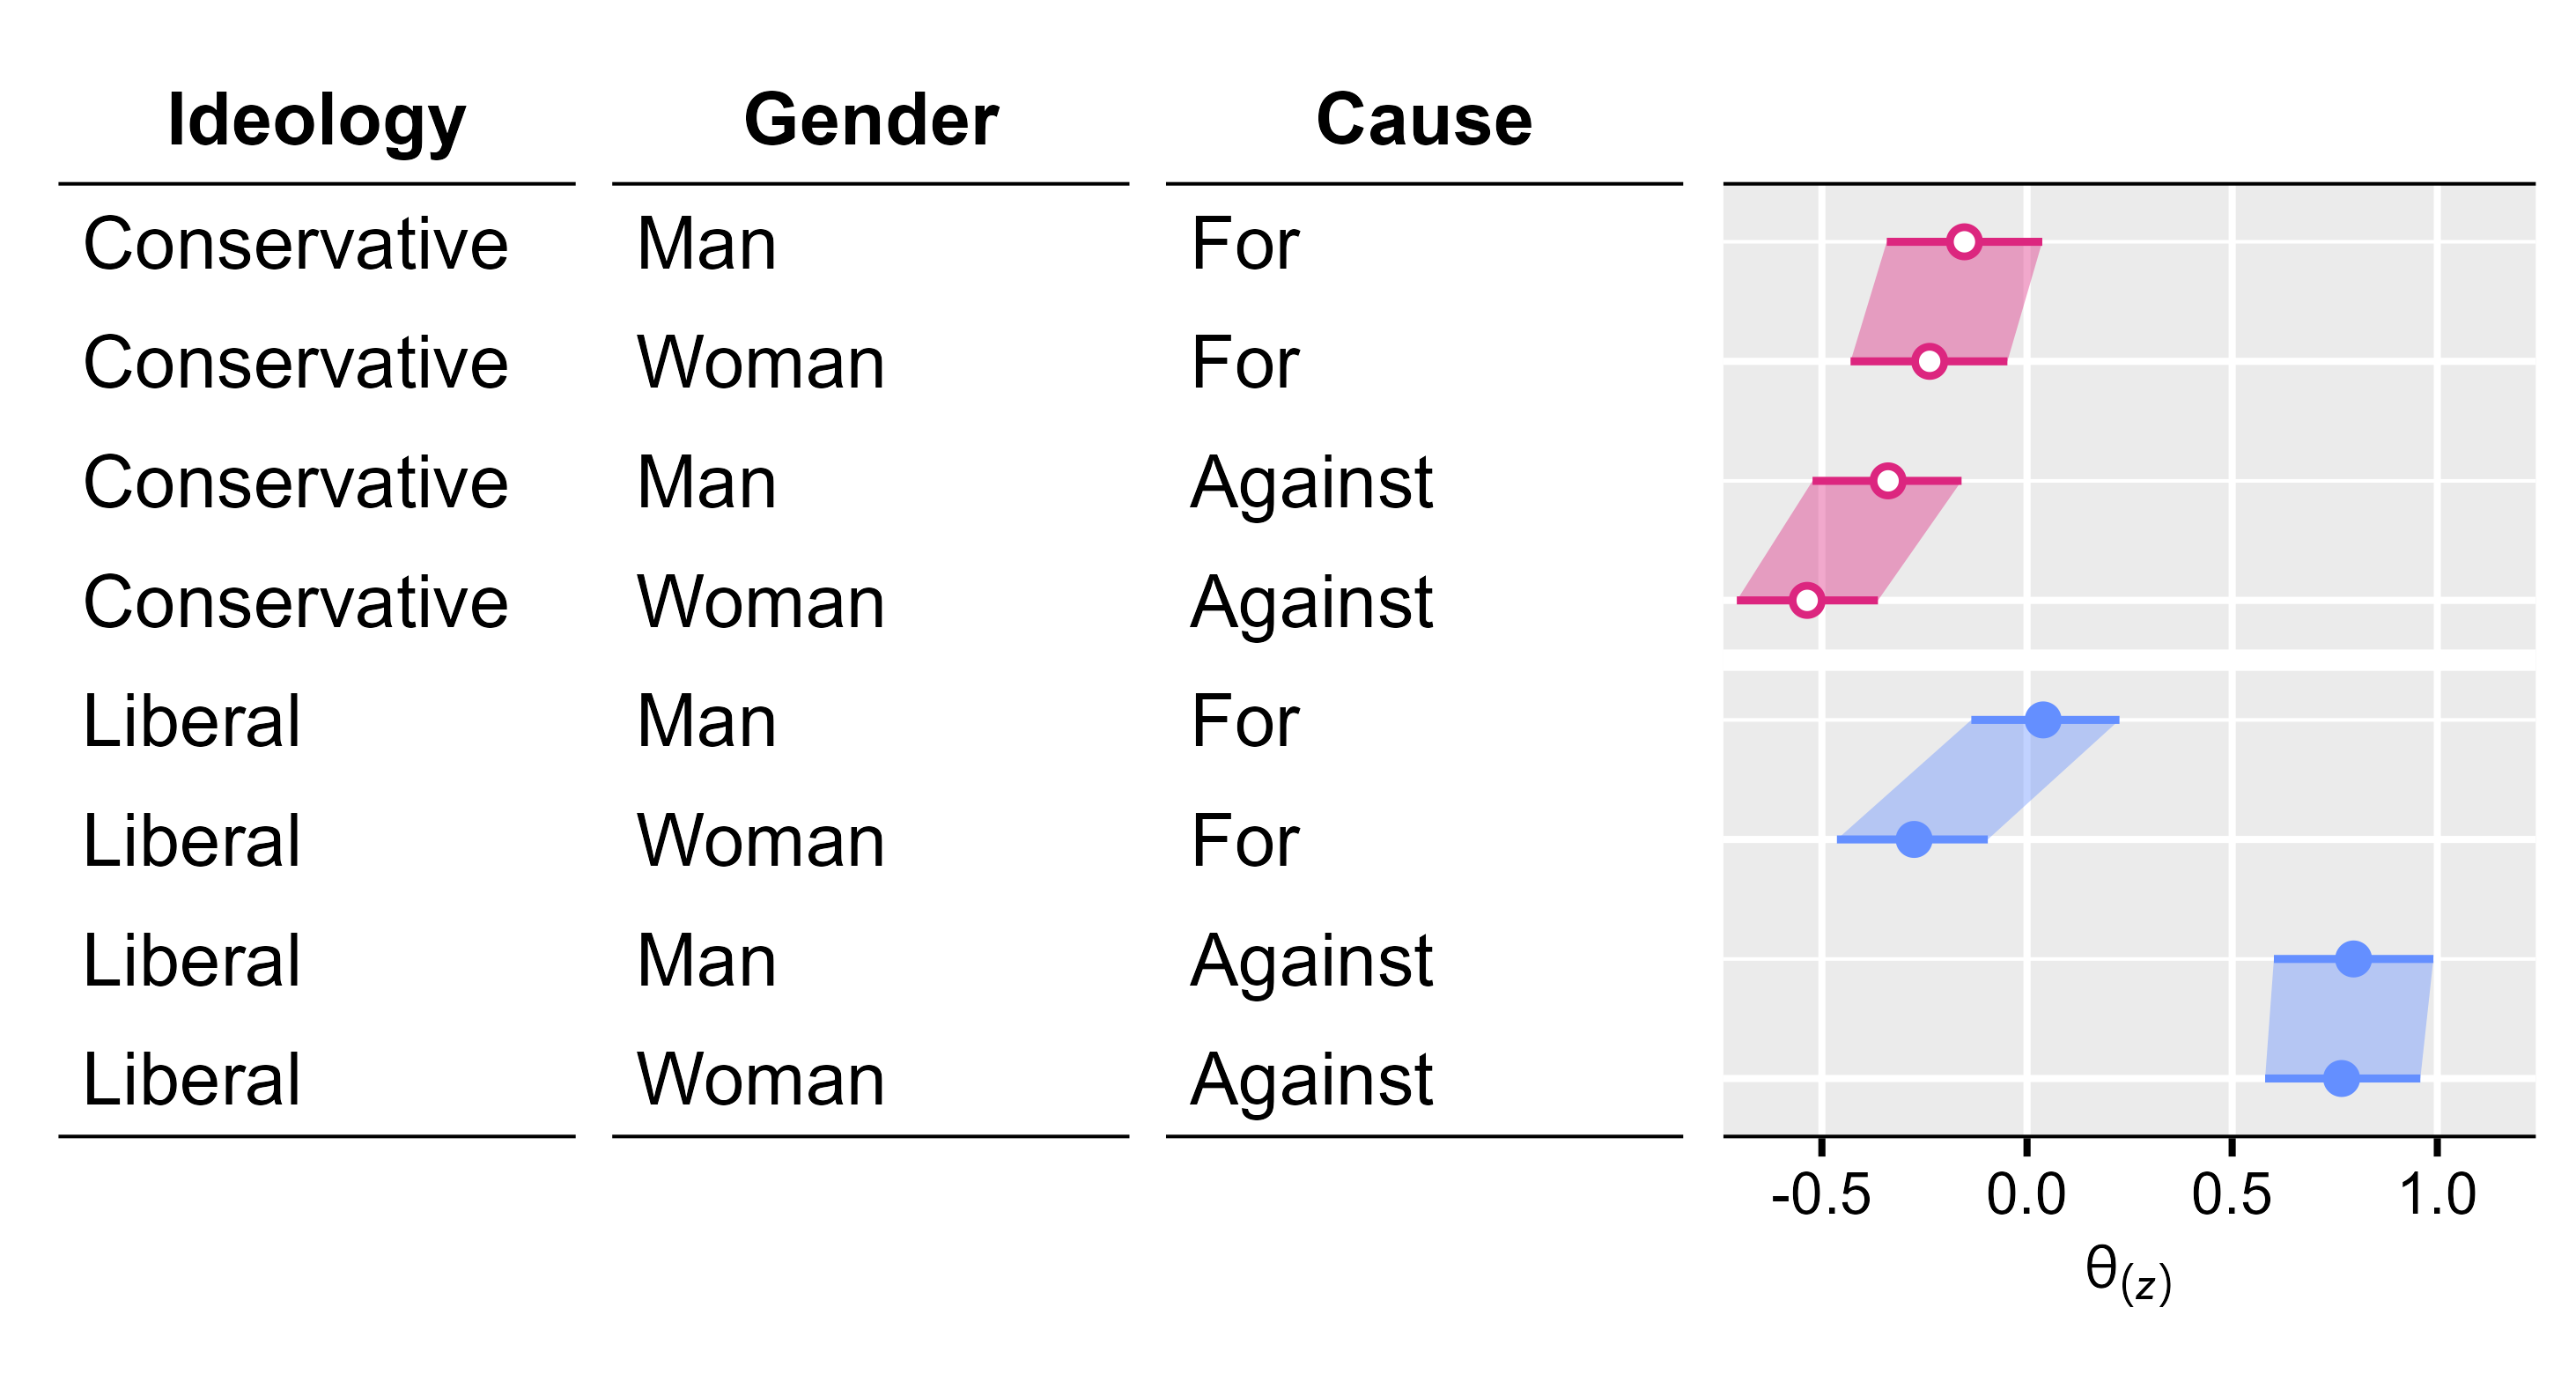
\includegraphics[scale=1]{../Experiment 3/figures/figure-6}
\caption*{\textit{Note.} Results show the estimated \textit{z}-standardized tendency ($\theta_{(z)}$) to consider more controversial actions acceptable means to protest for or against restricting abortion as a function of the participants' ideology and gender.}
\label{fig:f6}
\end{figure*}

To test our hypotheses, we used a two-parameter logistic item response
theory model, identical to the one used in Experiment 2, to estimate how
likely participants were to consider each action an acceptable means of
protest as a function of the protesters' cause and of the participants'
gender and ideology. Figure \ref{fig:f6} shows the results of our
preregistered analyses.

As in Experiments 1 and 2, we found evidence for ideology-based double
standards: Conservative participants considered the same protest actions
to be more acceptable, on average, when protesters \emph{supported}
restricting abortion (\(d = 0.24, [0.07, 0.43]\)) while liberal
participants considered the same protest actions to be more acceptable
when protesters \emph{opposed} restricting abortion
(\(d = 0.90, [0.72, 1.08]\)). This double standard was more pronounced
among liberal participants (\(d = 0.66, [0.41, 0.92]\)). In this way,
Experiment 3 provided evidence for both ideological symmetry and
asymmetry in judging collective action for and against restricting
abortion.

We found some evidence for gender-based double standards: Female
participants considered protest actions \emph{against} restricting
abortion to be more acceptable, on average, than male participants or
protest actions \emph{for} restricting abortion
(\(d = 0.14, [0.00, 0.29]\)). This pattern was, however, overshadowed by
stronger ideology-based double standards that were consistent across
subsamples: Conservative women (\(d = 0.30, [0.04, 0.55]\)) and, to a
lesser extent, conservative men (\(d = 0.19, [-0.07, 0.46]\)) considered
the same protest actions to be more acceptable when protesters
\emph{supported} restricting abortion and both liberal women
(\(d = 1.04, [0.78, 1.32]\)) and liberal men
(\(d = 0.76, [0.49, 1.03]\)) considered the same protest actions to be
more acceptable when protesters \emph{opposed} restricting abortion. In
this way, Experiment 3 provided more consistent evidence for
ideology-based than for gender-based double standards in judging
collective action. Across conditions, men tended to consider more
protest actions acceptable than women (\(d = 0.16, [0.02, 0.30]\)).

\hypertarget{non-preregistered-analyses-2}{%
\subsubsection{Non-Preregistered
Analyses}\label{non-preregistered-analyses-2}}

We explored whether group identification moderated participants'
judgments. We found, however, that gender identification neither
affected how women judged protesters opposing
(\(\beta_{xy} = -0.04, [-0.14, 0.07]\)) or supporting
(\(\beta_{xy} = -0.06, [-0.17, 0.03]\)) abortion restrictions nor how
men judged protesters opposing (\(\beta_{xy} = -0.05, [-0.14, 0.04]\))
or supporting (\(\beta_{xy} = -0.04, [-0.12, 0.06]\)) abortion
restrictions. Our non-preregistered analyses thus suggested that gender
identification did not moderate gender-based double standards in judging
collective action concerning reproductive rights.

\hypertarget{discussion-2}{%
\subsection{Discussion}\label{discussion-2}}

Experiment 3 tested for double standards in judging collective action
for and against restricting abortion in a sample balanced by gender and
political orientation. As hypothesized, participants judged the same
protest actions to be more acceptable when the protesters' cause aligned
with their ideological orientation. While participants in Experiment 2
judged protests opposing or supporting a progressive cause (defunding
police), participants in Experiment 3 considered protests opposing or
supporting a conservative cause (restricting abortion). As both
conservative and liberal participants judged protests for a cause
aligned with their ideological orientation to be more acceptable and as
this double standard was stronger among liberal participants, Experiment
3 provided evidence for both symmetry and asymmetry in ideology-based
double standards in judging collective action.

In contrast to Experiments 1--2, Experiment 3 provided some evidence for
group-based double standards distinct from ideology-based double
standards, although any gender differences in judging protests for or
against restricting abortion were overshadowed by more consistent
ideology-based double standards. Our finding that conservative women
considered collective action in support of restricting abortion to be
more acceptable while liberal women considered collective action in
opposition to restricting abortion to be more acceptable aligned with
Mikolajczak et al.'s (2022) argument that, by itself, gender identity is
too broad to explain support for collective action. Instead, we need to
consider the content of those identities---for example, identification
with feminism or with traditional women---to understand support for, and
opposition to, progressive and reactionary collective action.

\hypertarget{general-discussion}{%
\section{General Discussion}\label{general-discussion}}

Our research was motivated by real-world examples that seemed to suggest
that where people draw the line between acceptable and unacceptable
protest actions depends on \emph{who} the protesters are and \emph{what}
they are protesting---in other words, that there are double standards in
judging collective action. Our findings, however, showed that it is not
so simple.

Contradicting our hypothesis of group-based double standards,
participants in three preregistered experiments did not show consistent
ingroup bias in terms of social class when judging protests for workers'
rights (Experiment 1), in terms of race when judging protests for and
against defunding the police (Experiment 2), and in terms of gender when
judging protests for and against restricting abortion (Experiment 3).
Instead, we found that members of advantaged groups---middle-class
(Experiment 1), White (Experiment 2), and male (Experiment 3)
participants---tended to consider all protest actions more acceptable
than members of relatively disadvantaged groups. That is, our findings
showed that participants' judgements of protest actions depended on
their group memberships---but not in the directions implied by the
hypothesized group-based double standards.

Supporting our hypothesis of ideology-based double standards,
progressive participants who rejected system-justifying beliefs judged
the same controversial protest actions to be more acceptable when the
protesters' cause---for workers' rights (Experiment 1), for defunding
the police (Experiment 2), against restricting abortion (Experiment
3)---aligned with their own ideological position. While conservative
participants who endorsed system-justifying beliefs considered the same
actions somewhat more acceptable when protesters supported, rather than
opposed, restricting abortion (Experiment 3), they were more consistent
than liberal participants and considered all protest actions, for and
against defunding the police (Experiment 2), less acceptable than
progressive participants. In this way, our findings provided evidence
for asymmetrical ideology-based double standards.

In the remainder of this General Discussion, we discuss limiting
conditions on our findings as well as theoretical and practical
implications for understanding the often divided response to collective
action.

\hypertarget{limitations}{%
\subsection{Limitations}\label{limitations}}

Our research applied item response theory to judgments about collective
action to investigate whether where people draw the line between
acceptable and unacceptable means of protest depends on who the
protesters are and what they are protesting. In so doing, we moved the
distinction between normative and non-normative collective action from
the realm of the researcher's intuition into the realm of scientific
investigation, allowing us to test for double standards in judging
collective action.

Despite its strengths, our research has several limitations that
constrain the generalizability of our findings. First, our research
examined the hypothesized relationships for three political
causes---protecting workers' rights, defunding the police, restricting
abortion---and thus provided only limited evidence that our findings
generalize beyond those causes. Relying on few stimuli to establish an
effect threatens the validity and replicability of research findings and
constrains the generalizability of psychological research (Yarkoni,
2022). Future research should sample a wider range of causes to address
this pervasive but often ignored problem (Judd et al., 2012). This is
particularly important when studying collective action as recent
theorizing (Jost et al., 2017) and research (Osborne et al., 2019)
highlighted the importance of differentiating between progressive and
conservative causes. Second, our research was based on samples from two
Western, Educated, Industrialized, Rich, and Democratic (WEIRD, Henrich
et al., 2010) contexts---the United Kingdom and the United
States---which limits the cross-cultural generalizability of our
findings.

\hypertarget{implications}{%
\subsection{Implications}\label{implications}}

\hypertarget{theoretical-implications}{%
\subsubsection{Theoretical
Implications}\label{theoretical-implications}}

Growing evidence shows that, in many situations, observers apply a more
lenient standard when judging moral transgressions by ingroup members
(Abrams et al., 2013; Endevelt et al., 2021). And yet, our findings
suggested that, unlike judgments in other domains, judgments about
collective action are not subject to double standards based on ascribed
group memberships such as class, race, or gender. We did not find
evidence for those double standards even though we examined social
categories that are central to most people's identities, even when we
considered only highly identified group members, and even though
participants' reactions to the manipulation showed that, at least in
Experiments 1--2, they understood the protesters' causes in
ingroup--outgroup terms.

Instead, our findings showed that progressives and, to a lesser extent,
conservatives judge the same controversial protest actions to be more
acceptable when the protesters' cause aligns with their own ideological
position. We consider social, political, and moral psychological
explanations for the observed ideology-based double standards.

First, we might understand ideology-based double standards as an
expression of ingroup bias based on partisan identities (Finkel et al.,
2020; Harris et al., 2022). This explanation aligns with Verkuyten et
al.'s (2022) finding that participants were more tolerant of
transgressive protest actions when taken by their most-liked, rather
than their least-liked, political group. An identity-based account,
however, implies that both conservatives and progressives would show
ingroup bias and, therefore, cannot explain the observed asymmetry in
the two groups' judgements.

Second, we might explain ideology-based double standards, as we have
done so far, as resulting from conservatives being motivated to defend
the system, progressives being motivated to challenge the system, and
both being motivated to support collective action to those effects (Jost
et al., 2017; Osborne et al., 2019). An ideology-based account could
also explain the asymmetry in how progressives and conservatives judged
collective action for various causes. Political conservatism can be
understood as uniting two motives, to resist social change and to
maintain social inequality (Jost et al., 2003; Jost, 2021). If
conservatives perceive disruptive protest actions as inherently
threatening to the social order, they will be motivated to condemn such
actions even when the protesters' cause supports the unequal status quo
(e.g., protesting \emph{against} defunding the police).

Lastly, we might consider that collective action, even in its
controversial forms, is not judged as a moral transgression (as in
previous research on identity-based double standards, e.g., Abrams et
al., 2013)---but is instead understood as a means to an end and judged
in relation to its end (``the end justifies the means''). Their
different moral concerns (Graham et al., 2009; Kivikangas et al., 2021)
might lead progressives and conservatives to see their support of
certain causes as a fundamental matter of right or wrong (Skitka et al.,
2021) and, by thus moralizing those causes, to accept more extreme means
to achieving them. This explanation aligns with Richardson and Conway's
(2022) finding that moral concerns explained why liberals rated
protesting for liberal causes as more moral than conservatives (and vice
versa). A values-based account could also explain why conservatives who,
more so than liberals, endorse moral concerns related to loyalty and
authority tend to reject disruptive protest actions even when the
protesters' cause otherwise aligns with their moral concerns.

Future research should, across different causes, contexts, and cultures,
seek to disentangle which of the proposed social, political, and moral
psychological processes best explains partisan differences in judging
collective action.

\hypertarget{practical-implications}{%
\subsubsection{Practical Implications}\label{practical-implications}}

Most broadly, our findings showed that, for many protest actions (e.g.,
blocking roads), there is no consensus on whether they are acceptable
means to advance a cause. This confirms our contention that the
distinction between normative and non-normative collective action should
be situated in the eye of the beholder. By developing an instrument for
measuring where people draw the line between acceptable and unacceptable
forms of collective action, we provide a paradigm that we hope will
stimulate research on when and why people differ in making this
distinction.

After all, this distinction is consequential. Research on how people
respond to collective action showed that disruptive yet non-violent
collective action might be most effective at gaining concessions from
those resistant to social change (Shuman et al., 2021, 2023). If, as our
research suggests, people believe that even non-violent actions are
unacceptable means to advance a cause they oppose, they might support
stifling dissent. This could explain why Republicans responded to Black
Lives Matter protests by seeking to further criminalize disruptive
protest (e.g., blocking highways, Quinton, 2021) that might be most
effective at challenging injustice. In this way, our research
complements, and adds to, the growing program of research on how people
respond to different kinds of collective action.

If people believe that even extreme actions are acceptable means to
advance a cause they support, especially if they moralize their support
for that cause (Mooijman et al., 2018), they might support violent
extremism. For example, 45\% of Republicans supported the storming of
the U.S. Capitol on January 6, 2021 (YouGov, 2021) even though it was
illegal, destructive, and violent. Recent research, most of it by
political scientists, investigated support for partisan violence (Kalmoe
\& Mason, 2022), albeit with mixed results (Westwood et al., 2022).
While our research focused on controversial but non-violent actions, we
encourage researchers to adapt our paradigm to investigate when and why
people apply different standards when judging violent and non-violent
collective action for different causes.

\hypertarget{conclusion}{%
\section{Conclusion}\label{conclusion}}

Opinion polls show deep divides not only about the ends of protests, but
also about the means of protest. For example, only 11\% of Republicans
and 29\% of White Americans---compared to 59\% of Democrats and 66\% of
Black Americans---considered kneeling during the national anthem---a
non-violent form of collective action---an appropriate means to protest
racist police violence (YouGov, 2017). Our research showed that, in
contrast to well-documented double standards in other domains, people do
not apply a different standard when judging collective action by members
of the same class, race or gender or for a cause aligned with their own
group's interests. Instead, our research demonstrated that progressives
and, less so, conservatives consider the same protest actions to be more
acceptable when the cause of the protest aligns with their own
ideological position.

\refsection

\begingroup

\noindent \setlength{\parindent}{-0.5in} \setlength{\leftskip}{0.5in}
\small

\hypertarget{refs}{}
\begin{CSLReferences}{1}{0}
\leavevmode\vadjust pre{\hypertarget{ref-abrams_double_2013}{}}%
Abrams, D., Randsley de Moura, G., \& Travaglino, G. A. (2013). A double
standard when group members behave badly: {Transgression} credit to
ingroup leaders. \emph{Journal of Personality and Social Psychology},
\emph{105}(5), 799--815. \url{https://doi.org/10.1037/a0033600}

\leavevmode\vadjust pre{\hypertarget{ref-atari_morality_2022}{}}%
Atari, M., Haidt, J., Graham, J., Koleva, S., Stevens, S. T., \&
Dehghani, M. (2022). Morality beyond the {WEIRD}: How the nomological
network of morality varies across cultures. \emph{PsyArXiv}.
\url{https://doi.org/10.31234/osf.io/q6c9r}

\leavevmode\vadjust pre{\hypertarget{ref-becker_virtual_2012}{}}%
Becker, J. C. (2012). Virtual special issue on theory and research on
collective action in the {European} {Journal} of {Social} {Psychology}
{[}{Editorial}{]}. \emph{European Journal of Social Psychology},
\emph{42}(1), 19--23. \url{https://doi.org/10.1002/ejsp.1839}

\leavevmode\vadjust pre{\hypertarget{ref-becker_dynamic_2015}{}}%
Becker, J. C., \& Tausch, N. (2015). A dynamic model of engagement in
normative and non-normative collective action: {Psychological}
antecedents, consequences, and barriers. \emph{European Review of Social
Psychology}, \emph{26}(1), 43--92.
\url{https://doi.org/10.1080/10463283.2015.1094265}

\leavevmode\vadjust pre{\hypertarget{ref-becker_committed_2011}{}}%
Becker, J. C., Tausch, N., Spears, R., \& Christ, O. (2011). Committed
dis(s)idents: {Participation} in radical collective action fosters
disidentification with the broader in-group but enhances political
identification. \emph{Personality and Social Psychology Bulletin},
\emph{37}(8), 1104--1116. \url{https://doi.org/10.1177/0146167211407076}

\leavevmode\vadjust pre{\hypertarget{ref-brewer_social_2007}{}}%
Brewer, M. B. (2007). The social psychology of intergroup relations:
Social categorization, ingroup bias, and outgroup prejudice. In A. W.
Kruglanski \& E. T. Higgins (Eds.), \emph{Social psychology: Handbook of
basic principles} (2nd ed., pp. 695--715). Guilford Press.

\leavevmode\vadjust pre{\hypertarget{ref-burkner_bayesian_2021}{}}%
Bürkner, P.-C. (2021). Bayesian item response modeling in {R} with brms
and {Stan}. \emph{Journal of Statistical Software}, \emph{100}(5).
\url{https://doi.org/10.18637/jss.v100.i05}

\leavevmode\vadjust pre{\hypertarget{ref-burkner_modelling_2020}{}}%
Bürkner, P.-C., \& Charpentier, E. (2020). Modelling monotonic effects
of ordinal predictors in {Bayesian} regression models. \emph{British
Journal of Mathematical and Statistical Psychology}, \emph{73}(3),
420--451. \url{https://doi.org/10.1111/bmsp.12195}

\leavevmode\vadjust pre{\hypertarget{ref-cohen_party_2003}{}}%
Cohen, G. L. (2003). Party over policy: The dominating impact of group
influence on political beliefs. \emph{Journal of Personality and Social
Psychology}, \emph{85}(5), 808--822.
\url{https://doi.org/10.1037/0022-3514.85.5.808}

\leavevmode\vadjust pre{\hypertarget{ref-demars_irt_2010}{}}%
DeMars, C. (2010). \emph{Item response theory}. Oxford University Press.

\leavevmode\vadjust pre{\hypertarget{ref-dunivin_black_2022}{}}%
Dunivin, Z. O., Yan, H. Y., Ince, J., \& Rojas, F. (2022). Black {Lives}
{Matter} protests shift public discourse. \emph{Proceedings of the
National Academy of Sciences}, \emph{119}(10), e2117320119.
\url{https://doi.org/10.1073/pnas.2117320119}

\leavevmode\vadjust pre{\hypertarget{ref-endevelt_everyone_2021}{}}%
Endevelt, K., Schori-Eyal, N., \& Halperin, E. (2021). Everyone should
get the same, but we should get more: Group entitlement and intergroup
moral double standard. \emph{Group Processes \& Intergroup Relations},
\emph{24}(3), 350--370. \url{https://doi.org/10.1177/1368430219896618}

\leavevmode\vadjust pre{\hypertarget{ref-feinberg_activists_2020}{}}%
Feinberg, M., Willer, R., \& Kovacheff, C. (2020). The activist's
dilemma: {Extreme} protest actions reduce popular support for social
movements. \emph{Journal of Personality and Social Psychology},
\emph{119}(5), 1086--1111. \url{https://doi.org/10.1037/pspi0000230}

\leavevmode\vadjust pre{\hypertarget{ref-finkel_political_2020}{}}%
Finkel, E. J., Bail, C. A., Cikara, M., Ditto, P. H., Iyengar, S., Klar,
S., Mason, L., McGrath, M. C., Nyhan, B., Rand, D. G., Skitka, L. J.,
Tucker, J. A., Van Bavel, J. J., Wang, C. S., \& Druckman, J. N. (2020).
Political sectarianism in {America}. \emph{Science}, \emph{370}(6516),
533--536. \url{https://doi.org/10.1126/science.abe1715}

\leavevmode\vadjust pre{\hypertarget{ref-foschi_double_2000}{}}%
Foschi, M. (2000). Double standards for competence: Theory and research.
\emph{Annual Review of Sociology}, \emph{26}(1), 21--42.
\url{https://doi.org/10.1146/annurev.soc.26.1.21}

\leavevmode\vadjust pre{\hypertarget{ref-cmdstanr_2021}{}}%
Gabry, J., \& Cesnovar, R. (2021). \emph{{cmdstanr}: {R} interface to
{CmdStan}} (Version 0.4.0). \url{https://mc-stan.org/cmdstanr}

\leavevmode\vadjust pre{\hypertarget{ref-gelman_why_2012}{}}%
Gelman, A., Hill, J., \& Yajima, M. (2012). Why we (usually) don't have
to worry about multiple comparisons. \emph{Journal of Research on
Educational Effectiveness}, \emph{5}(2), 189--211.
\url{https://doi.org/10.1080/19345747.2011.618213}

\leavevmode\vadjust pre{\hypertarget{ref-gelman_prior_2017}{}}%
Gelman, A., Simpson, D., \& Betancourt, M. (2017). The prior can often
only be understood in the context of the likelihood. \emph{Entropy},
\emph{19, 10}, 555. \url{https://doi.org/10.3390/e19100555}

\leavevmode\vadjust pre{\hypertarget{ref-graham_liberals_2009}{}}%
Graham, J., Haidt, J., \& Nosek, B. A. (2009). Liberals and
conservatives rely on different sets of moral foundations. \emph{Journal
of Personality and Social Psychology}, \emph{96}(5), 1029--1046.
\url{https://doi.org/10.1037/a0015141}

\leavevmode\vadjust pre{\hypertarget{ref-osborne_psychology_2022}{}}%
Harris, E., Pärnamets, P., Sternisko, A., Robertson, C., \& Van Bavel,
J. J. (2022). The psychology and neuroscience of partisanship. In D.
Osborne \& C. G. Sibley (Eds.), \emph{The {Cambridge} handbook of
political psychology} (pp. 50--67). Cambridge University Press.
\url{https://doi.org/10.1017/9781108779104.005}

\leavevmode\vadjust pre{\hypertarget{ref-henrich_weirdest_2010}{}}%
Henrich, J., Heine, S. J., \& Norenzayan, A. (2010). The weirdest people
in the world? \emph{Behavioral and Brain Sciences}, \emph{33}(2-3),
61--135. \url{https://doi.org/10.1017/S0140525X10000725}

\leavevmode\vadjust pre{\hypertarget{ref-hewstone_ultimate_1990}{}}%
Hewstone, M. (1990). The {``ultimate attribution error''}? {A} review of
the literature on intergroup causal attribution. \emph{European Journal
of Social Psychology}, \emph{20}(4), 311--335.
\url{https://doi.org/10.1002/ejsp.2420200404}

\leavevmode\vadjust pre{\hypertarget{ref-ho_nature_2015}{}}%
Ho, A. K., Sidanius, J., Kteily, N., Sheehy-Skeffington, J., Pratto, F.,
Henkel, K. E., Foels, R., \& Stewart, A. L. (2015). The nature of social
dominance orientation: {Theorizing} and measuring preferences for
intergroup inequality using the new {SDO}-7 scale. \emph{Journal of
Personality and Social Psychology}, \emph{109}(6), 1003--1028.
\url{https://doi.org/10.1037/pspi0000033}

\leavevmode\vadjust pre{\hypertarget{ref-jimenez-moya_by_2015}{}}%
Jiménez-Moya, G., Spears, R., Rodríguez-Bailón, R., \& Lemus, S. de.
(2015). By any means necessary? {When} and why low group identification
paradoxically predicts radical collective action: Predicting radical
collective action. \emph{Journal of Social Issues}, \emph{71}(3),
517--535. \url{https://doi.org/10.1111/josi.12126}

\leavevmode\vadjust pre{\hypertarget{ref-jost_theory_2020}{}}%
Jost, J. T. (2020). \emph{A theory of system justification}. Harvard
University Press.

\leavevmode\vadjust pre{\hypertarget{ref-jost_left_2021}{}}%
Jost, J. T. (2021). \emph{Left and right: The psychological significance
of a political distinction}. Oxford University Press.

\leavevmode\vadjust pre{\hypertarget{ref-jost_decade_2004}{}}%
Jost, J. T., Banaji, M. R., \& Nosek, B. A. (2004). A decade of system
justification theory: Accumulated evidence of conscious and unconscious
bolstering of the status quo. \emph{Political Psychology}, \emph{25}(6),
881--919. \url{https://doi.org/10.1111/j.1467-9221.2004.00402.x}

\leavevmode\vadjust pre{\hypertarget{ref-jost_missing_2017}{}}%
Jost, J. T., Becker, J., Osborne, D., \& Badaan, V. (2017). Missing in
(collective) action: Ideology, system justification, and the
motivational antecedents of two types of protest behavior. \emph{Current
Directions in Psychological Science}, \emph{26}(2), 99--108.
\url{https://doi.org/10.1177/0963721417690633}

\leavevmode\vadjust pre{\hypertarget{ref-jost_political_2003}{}}%
Jost, J. T., Glaser, J., Kruglanski, A. W., \& Sulloway, F. J. (2003).
Political conservatism as motivated social cognition.
\emph{Psychological Bulletin}, \emph{129}(3), 339--375.
\url{https://doi.org/10.1037/0033-2909.129.3.339}

\leavevmode\vadjust pre{\hypertarget{ref-jost_exposure_2005}{}}%
Jost, J. T., \& Kay, A. C. (2005). Exposure to benevolent sexism and
complementary gender stereotypes: Consequences for specific and diffuse
forms of system justification. \emph{Journal of Personality and Social
Psychology}, \emph{88}(3), 498--509.
\url{https://doi.org/10.1037/0022-3514.88.3.498}

\leavevmode\vadjust pre{\hypertarget{ref-judd_treating_2012}{}}%
Judd, C. M., Westfall, J., \& Kenny, D. A. (2012). Treating stimuli as a
random factor in social psychology: {A} new and comprehensive solution
to a pervasive but largely ignored problem. \emph{Journal of Personality
and Social Psychology}, \emph{103}(1), 54--69.
\url{https://doi.org/10.1037/a0028347}

\leavevmode\vadjust pre{\hypertarget{ref-kalmoe_radical_2022}{}}%
Kalmoe, N. P., \& Mason, L. (2022). \emph{Radical {American}
partisanship: Mapping violent hostility, its causes, and the
consequences for democracy}. The University of Chicago Press.

\leavevmode\vadjust pre{\hypertarget{ref-kay_complementary_2003}{}}%
Kay, A. C., \& Jost, J. T. (2003). Complementary justice: Effects of
"poor but happy" and "poor but honest" stereotype exemplars on system
justification and implicit activation of the justice motive.
\emph{Journal of Personality and Social Psychology}, \emph{85}(5),
823--837. \url{https://doi.org/10.1037/0022-3514.85.5.823}

\leavevmode\vadjust pre{\hypertarget{ref-kivikangas_moral_2021}{}}%
Kivikangas, J. M., Fernández-Castilla, B., Järvelä, S., Ravaja, N., \&
Lönnqvist, J.-E. (2021). Moral foundations and political orientation:
{Systematic} review and meta-analysis. \emph{Psychological Bulletin},
\emph{147}(1), 55--94. \url{https://doi.org/10.1037/bul0000308}

\leavevmode\vadjust pre{\hypertarget{ref-leach_social_2017}{}}%
Leach, C. W., \& Allen, A. M. (2017). The social psychology of the
{Black Lives Matter} meme and movement. \emph{Current Directions in
Psychological Science}, \emph{26}(6), 543--547.
\url{https://doi.org/10.1177/0963721417719319}

\leavevmode\vadjust pre{\hypertarget{ref-leach_understanding_2022}{}}%
Leach, C. W., \& Teixeira, C. P. (2022). Understanding sentiment toward
{``{Black Lives Matter}.''} \emph{Social Issues and Policy Review},
\emph{16}(1), 3--32. \url{https://doi.org/10.1111/sipr.12084}

\leavevmode\vadjust pre{\hypertarget{ref-mendoza_for_2014}{}}%
Mendoza, S. A., Lane, S. P., \& Amodio, D. M. (2014). For members only:
Ingroup punishment of fairness norm violations in the ultimatum game.
\emph{Social Psychological and Personality Science}, \emph{5}(6),
662--670. \url{https://doi.org/10.1177/1948550614527115}

\leavevmode\vadjust pre{\hypertarget{ref-mikolajczak_women_2022}{}}%
Mikolajczak, G., Becker, J. C., \& Iyer, A. (2022). Women who challenge
or defend the status quo: {Ingroup} identities as predictors of
progressive and reactionary collective action. \emph{European Journal of
Social Psychology}. \url{https://doi.org/10.1002/ejsp.2842}

\leavevmode\vadjust pre{\hypertarget{ref-mooijman_moralization_2018}{}}%
Mooijman, M., Hoover, J., Lin, Y., Ji, H., \& Dehghani, M. (2018).
Moralization in social networks and the emergence of violence during
protests. \emph{Nature Human Behaviour}, \emph{2}(6), 389--396.
\url{https://doi.org/10.1038/s41562-018-0353-0}

\leavevmode\vadjust pre{\hypertarget{ref-osborne_protesting_2019}{}}%
Osborne, D., Jost, J. T., Becker, J. C., Badaan, V., \& Sibley, C. G.
(2019). Protesting to challenge or defend the system? {A} system
justification perspective on collective action. \emph{European Journal
of Social Psychology}, \emph{49}(2), 244--269.
\url{https://doi.org/10.1002/ejsp.2522}

\leavevmode\vadjust pre{\hypertarget{ref-acceptable}{}}%
Oxford Advanced Learner's Dictionary. (n.d.). \emph{Acceptable}.
\url{https://www.oxfordlearnersdictionaries.com/us/definition/english/acceptable}

\leavevmode\vadjust pre{\hypertarget{ref-pettigrew_ultimate_1979}{}}%
Pettigrew, T. F. (1979). The ultimate attribution error: Extending
{Allport}'s cognitive analysis of prejudice. \emph{Personality and
Social Psychology Bulletin}, \emph{5}(4), 461--476.
\url{https://doi.org/10.1177/014616727900500407}

\leavevmode\vadjust pre{\hypertarget{ref-pinsof_strange_2023}{}}%
Pinsof, D., Sears, D. O., \& Haselton, M. G. (2023). Strange bedfellows:
The alliance theory of political belief systems. \emph{Psychological
Inquiry}, \emph{34}(3), 139--160.
\url{https://doi.org/10.1080/1047840X.2023.2274433}

\leavevmode\vadjust pre{\hypertarget{ref-pinto_membership_2010}{}}%
Pinto, I. R., Marques, J. M., Levine, J. M., \& Abrams, D. (2010).
Membership status and subjective group dynamics: Who triggers the black
sheep effect? \emph{Journal of Personality and Social Psychology},
\emph{99}(1), 107--119. \url{https://doi.org/10.1037/a0018187}

\leavevmode\vadjust pre{\hypertarget{ref-pew_republicans_2021}{}}%
Quinton, S. (2021). Republicans respond to {Black Lives Matter} with
anti-protest bills. \emph{Pew Charitable Trusts}.
\url{https://pew.org/3rhdGYw}

\leavevmode\vadjust pre{\hypertarget{ref-reimer_identity_2022}{}}%
Reimer, N. K., Schmid, K., Hewstone, M., \& Al Ramiah, A. (2022).
Self-categorization and social identification: Making sense of us and
them. In D. Chadee (Ed.), \emph{Theories in social psychology} (2nd ed.,
pp. 273--295). Wiley-Blackwell.

\leavevmode\vadjust pre{\hypertarget{ref-richardson_standing_2022}{}}%
Richardson, I., \& Conway, P. (2022). Standing up or giving up? {Moral}
foundations mediate political differences in evaluations of {BLACK}
{LIVES} {MATTER} and other protests. \emph{European Journal of Social
Psychology}, \emph{52}(3), 553--569.
\url{https://doi.org/10.1002/ejsp.2837}

\leavevmode\vadjust pre{\hypertarget{ref-ryan_reconsidering_2014}{}}%
Ryan, T. J. (2014). Reconsidering moral issues in politics. \emph{The
Journal of Politics}, \emph{76}(2), 380--397.
\url{https://doi.org/10.1017/S0022381613001357}

\leavevmode\vadjust pre{\hypertarget{ref-samejima_graded_1997}{}}%
Samejima, F. (1997). Graded response model. In W. J. van der Linden \&
R. K. Hambleton (Eds.), \emph{Handbook of modern item response theory}
(pp. 85--100). Springer.

\leavevmode\vadjust pre{\hypertarget{ref-sharp_nonviolent_1973}{}}%
Sharp, G. (1973). \emph{The politics of nonviolent action}. Porter
Sargent.

\leavevmode\vadjust pre{\hypertarget{ref-shuman_when_2023}{}}%
Shuman, E., Goldenberg, A., Saguy, T., Halperin, E., \& Van Zomeren, M.
(2023). When are social protests effective? \emph{Trends in Cognitive
Sciences}, S1364661323002619.
\url{https://doi.org/10.1016/j.tics.2023.10.003}

\leavevmode\vadjust pre{\hypertarget{ref-shuman_disrupting_2021}{}}%
Shuman, E., Saguy, T., van Zomeren, M., \& Halperin, E. (2021).
Disrupting the system constructively: {Testing} the effectiveness of
nonnormative nonviolent collective action. \emph{Journal of Personality
and Social Psychology}, \emph{121}(4), 819--841.
\url{https://doi.org/10.1037/pspi0000333}

\leavevmode\vadjust pre{\hypertarget{ref-skitka_psychology_2021}{}}%
Skitka, L. J., Hanson, B. E., Morgan, G. S., \& Wisneski, D. C. (2021).
The psychology of moral conviction. \emph{Annual Review of Psychology},
\emph{72}(1), 347--366.
\url{https://doi.org/10.1146/annurev-psych-063020-030612}

\leavevmode\vadjust pre{\hypertarget{ref-cmdstan_2021}{}}%
Stan Development Team. (2021). \emph{Stan modeling language users guide
and reference manual} (Version 2.27.0). \url{http://mc-stan.org/}

\leavevmode\vadjust pre{\hypertarget{ref-tajfel_integrative_1979}{}}%
Tajfel, H., \& Turner, J. C. (1979). An integrative theory of intergroup
conflict. In W. G. Austin \& S. Worchel (Eds.), \emph{The psychology of
intergroup relations} (pp. 33--48). Brooks/Cole.

\leavevmode\vadjust pre{\hypertarget{ref-teixeira_white_2022}{}}%
Teixeira, C. P., Leach, C. W., \& Spears, R. (2022). White {Americans}'
belief in systemic racial injustice and in-group identification affect
reactions to ({peaceful} vs. {destructive}) {``{Black Lives Matter}''}
protest. \emph{Psychology of Violence}, \emph{12}(4), 280--292.
\url{https://doi.org/10.1037/vio0000425}

\leavevmode\vadjust pre{\hypertarget{ref-teixeira_is_2020}{}}%
Teixeira, C. P., Spears, R., \& Yzerbyt, V. Y. (2020). Is {Martin}
{Luther} {King} or {Malcolm} {X} the more acceptable face of protest?
{High}-status groups' reactions to low-status groups' collective action.
\emph{Journal of Personality and Social Psychology}, \emph{118}(5),
919--944. \url{https://doi.org/10.1037/pspi0000195}

\leavevmode\vadjust pre{\hypertarget{ref-valdesolo_moral_2007}{}}%
Valdesolo, P., \& DeSteno, D. (2007). Moral hypocrisy: Social groups and
the flexibility of virtue. \emph{Psychological Science}, \emph{18}(8),
689--690. \url{https://doi.org/10.1111/j.1467-9280.2007.01961.x}

\leavevmode\vadjust pre{\hypertarget{ref-van_zomeren_building_2016}{}}%
van Zomeren, M. (2016). Building a tower of babel? {Integrating} core
motivations and features of social structure into the political
psychology of political action. \emph{Political Psychology}, \emph{37},
87--114. \url{https://doi.org/10.1111/pops.12322}

\leavevmode\vadjust pre{\hypertarget{ref-verkuyten_intolerance_2022}{}}%
Verkuyten, M., Adelman, L., \& Yogeeswaran, K. (2022). Intolerance of
transgressive protest actions: The differential roles of deontological
and utilitarian morality. \emph{Personality and Social Psychology
Bulletin}. \url{https://doi.org/10.1177/01461672221099709}

\leavevmode\vadjust pre{\hypertarget{ref-westwood_current_2022}{}}%
Westwood, S. J., Grimmer, J., Tyler, M., \& Nall, C. (2022). Current
research overstates {American} support for political violence.
\emph{Proceedings of the National Academy of Sciences}, \emph{119}(12),
e2116870119. \url{https://doi.org/10.1073/pnas.2116870119}

\leavevmode\vadjust pre{\hypertarget{ref-wright_responding_1990}{}}%
Wright, S. C., Taylor, D. M., \& Moghaddam, F. M. (1990). Responding to
membership in a disadvantaged group: From acceptance to collective
protest. \emph{Journal of Personality and Social Psychology},
\emph{58}(6), 994--1003.
\url{https://doi.org/10.1037/0022-3514.58.6.994}

\leavevmode\vadjust pre{\hypertarget{ref-yarkoni_generalizability_2022}{}}%
Yarkoni, T. (2022). The generalizability crisis. \emph{Behavioral and
Brain Sciences}, \emph{45}, e1.
\url{https://doi.org/10.1017/S0140525X20001685}

\leavevmode\vadjust pre{\hypertarget{ref-yougov_nfl_2017}{}}%
YouGov. (2017). \emph{{HuffPost: NFL} {(Sept. 25--26, 2017)}} {[}Data
set{]}. \url{https://perma.cc/3Q3V-4GC4}

\leavevmode\vadjust pre{\hypertarget{ref-yougov_police_2020}{}}%
YouGov. (2020). \emph{{HuffPost}: Police reform {(Dec. 3--6, 2020)}}
{[}Data set{]}. \url{https://perma.cc/JH5P-3W3K}

\leavevmode\vadjust pre{\hypertarget{ref-yougov_capitol_2021}{}}%
YouGov. (2021). \emph{Capitol protest {(Jan. 6, 2021)}} {[}Data set{]}.
\url{https://perma.cc/YG99-EUYX}

\end{CSLReferences}

\endgroup

\newpage

\setcounter{table}{0}
\renewcommand{\thetable}{A\arabic{table}}

\begin{table*}

\section{Appendix A}

\caption{List of protest actions used in Experiment 1}
\small
\begin{tabularx}{\linewidth}{rXr}
\addlinespace
\toprule
\# & Action & Pr\\
\midrule
1 & participate in a public meeting of representatives and elected officials & 97\%\\
2 & hold meetings to inform the public & 96\%\\
3 & make a public speech & 96\%\\
4 & hold meetings to influence the public & 93\%\\
5 & attend or organise a protest march & 93\%\\
6 & attend or organise a protest rally & 92\%\\
7 & use social media (e.g., Facebook, Twitter, Instagram) to influence the public & 92\%\\
8 & do not buy goods or services from companies who support the bill (consumers' boycott) & 92\%\\
9 & paste up posters with political messages in places where it is allowed and encouraged & 89\%\\
10 & join or form a group of activists who oppose the bill & 87\%\\
11 & refuse to accept honours or awards in protest & 82\%\\
12 & donate to political parties who oppose the bill & 80\%\\
13 & refuse to work (strike) & 80\%\\
14 & pay for adverts on social media (e.g., Facebook, Twitter, Instagram) to influence public opinion & 78\%\\
15 & donate to activist groups who oppose the bill & 77\%\\
16 & visit people in their homes to convince them about the issue (canvassing, door knocking) & 54\%\\
17 & stand or sit in a building and refuse to leave (stand-in, sit-in) & 51\%\\
18 & refuse to honour national symbols and traditions (e.g., refusing to sing the national anthem) until the bill is abandoned & 47\%\\
19 & enter and refuse to leave a building (occupation) & 38\%\\
20 & paste up posters with political messages in places where it is not allowed or encouraged & 35\%\\
21 & disrupt traffic (e.g., blocking roads) & 22\%\\
22 & refuse to cooperate with the police and other government agencies & 19\%\\
23 & mock or insult individuals who support the bill & 14\%\\
24 & spray paint political messages in public places & 14\%\\
25 & deface flags or other national symbols & 12\%\\
\bottomrule
\end{tabularx}
\caption*{\textit{Note.} Actions are ordered by the proportion of participants, across all conditions, who considered it to be an acceptable means of protest in Experiment 1.}

\end{table*}

\setcounter{table}{0}
\renewcommand{\thetable}{B\arabic{table}}

\begin{table*}

\section{Appendix B}

\caption{List of protest actions used in Experiment 2}
\small
\begin{tabularx}{\linewidth}{rXr}
\addlinespace
\toprule
\# & Action & Pr\\
\midrule
1 & make a public speech & 94\%\\
2 & \textit{hand out flyers, leaflets, or pamphlets} & 93\%\\
3 & use social media (e.g., Facebook, Twitter, Instagram) to influence the public & 91\%\\
4 & hold meetings to influence the public & 91\%\\
5 & paste up posters with political messages in places where it is allowed and encouraged & 91\%\\
6 & attend or organise a protest march & 91\%\\
7 & donate to activist groups & 89\%\\
8 & join or form a group of activists & 89\%\\
9 & \textit{wear or display political symbols (e.g., patches, flags, bumper stickers)} & 86\%\\
10 & refuse to buy goods or services from companies that advocate [against/for] defunding the police (boycott) & 85\%\\
11 & pay for adverts on social media (e.g., Facebook, Twitter, Instagram) to influence public opinion & 83\%\\
12 & donate to politicians who advocate [for/against] defunding the police & 82\%\\
13 & refuse to accept honors or awards in protest & 80\%\\
14 & refuse to work (strike) & 61\%\\
15 & visit people in their homes to convince them about the issue (canvassing, door knocking) & 61\%\\
16 & stand or sit in a building and refuse to leave (stand-in, sit-in) & 55\%\\
17 & \textit{attend a protest march even though it might turn violent} & 44\%\\
18 & \textit{attend a protest march even though it might be unlawful} & 42\%\\
19 & \textit{attend a protest march while carrying a firearm (where legal)} & 35\%\\
20 & enter and refuse to leave a building (occupation) & 34\%\\
21 & paste up posters with political messages in places where it is not allowed or encouraged & 29\%\\
22 & \textit{refuse to pay fees, fines, or taxes in protest} & 29\%\\
23 & disrupt traffic (e.g., blocking roads) & 25\%\\
24 & spray paint political messages in public places & 23\%\\
25 & mock or insult individuals who are [against/for] defunding the police & 15\%\\
\bottomrule
\end{tabularx}
\caption*{\textit{Note.} Actions are ordered by the proportion of participants, across all conditions, who considered it to be an acceptable means of protest in Experiment 2. Actions in \textit{italics} replaced actions used in Experiment 1 that were either redundant or did not fit the context of Experiment 2.}

\end{table*}

\setcounter{table}{0}
\renewcommand{\thetable}{C\arabic{table}}

\begin{table*}

\section{Appendix C}

\caption{List of protest actions used in Experiment 3}
\small
\begin{tabularx}{\linewidth}{rXr}
\addlinespace
\toprule
\# & Action & Pr\\
\midrule
1 & make a public speech & 94\%\\
2 & hand out flyers, leaflets, or pamphlets & 92\%\\
3 & wear or display political symbols (e.g., patches, flags, bumper stickers) & 92\%\\
4 & hold meetings to influence the public & 92\%\\
5 & attend or organise a protest march & 91\%\\
6 & use social media (e.g., Facebook, Twitter, Instagram) to influence the public & 91\%\\
7 & donate to activist groups & 90\%\\
8 & refuse to buy goods or services from companies that advocate [against/for] restricting or banning abortion (boycott) & 90\%\\
9 & paste up posters with political messages in places where it is allowed and encouraged & 90\%\\
10 & join or form a group of activists & 90\%\\
11 & donate to politicians who advocate [for/against] restricting or banning abortion & 89\%\\
12 & pay for adverts on social media (e.g., Facebook, Twitter, Instagram) to influence public opinion & 84\%\\
13 & refuse to accept honors or awards in protest & 82\%\\
14 & refuse to work (strike) & 56\%\\
15 & visit people in their homes to convince them about the issue (canvassing, door knocking) & 50\%\\
16 & stand or sit in a building and refuse to leave (stand-in, sit-in) & 41\%\\
17 & attend a protest march even though it might be unlawful & 40\%\\
18 & \textit{protest outside the homes of politicians who advocate [against/for] restricting or banning abortion} & 40\%\\
19 & attend a protest march even though it might turn violent & 40\%\\
20 & paste up posters with political messages in places where it is not allowed or encouraged & 26\%\\
21 & enter and refuse to leave a building (occupation) & 25\%\\
22 & refuse to pay fees, fines, or taxes in protest & 23\%\\
23 & mock or insult individuals who are [against/for] restricting or banning abortion & 20\%\\
24 & spray paint political messages in public places & 15\%\\
25 & disrupt traffic (e.g., blocking roads) & 12\%\\
\bottomrule
\end{tabularx}
\caption*{\textit{Note.} Actions are ordered by the proportion of participants, across all conditions, who considered it to be an acceptable means of protest in Experiment 3. Action in \textit{italics} replaced an action used in Experiment 2 because it better fit the context of Experiment 3.}

\end{table*}

\end{document}
